
%use mybib.bib for bibliography. bibtex is used for bibliography
%\documentclass[journal,12pt,onecolumn]{IEEEtran}
\documentclass[Journal]{IEEEtran}
\usepackage[utf8]{inputenc}
\usepackage{graphicx}
\usepackage{cite}
\usepackage{longtable}
\usepackage{amsmath}
\usepackage{multirow}
\usepackage{multicol}
\usepackage{wrapfig}
\usepackage{float}
%\usepackage[section]{placeins}
%\usepackage{subcaption}
\usepackage{array}
\usepackage[export]{adjustbox}
\usepackage{tabu}
\usepackage{tabularx}
\usepackage{listings}
\usepackage{siunitx}
\usepackage{siunitx}
\usepackage{ wasysym }
\usepackage[usenames, dvipsnames]{color}


%%%%%%%%%%%%%%%%%%%%%%%%%%%%%%%%%%%%%%%%%%%%%%%%%%%%%


\ifCLASSINFOpdf

\else

\fi


\hyphenation{op-tical net-works semi-conduc-tor}


\begin{document}

\title{Coordinated Voltage Control of Distribution System Containing Inverter Interfaced Distributed Generation}

\author{\IEEEauthorblockN{Alvi Newaz\IEEEauthorrefmark{1},
Juan Ospina\IEEEauthorrefmark{0}, M. Omar Faruque\IEEEauthorrefmark{0}}
\IEEEauthorblockA{\\The Department of Electrical and Computer Engineering at the FAMU-FSU College of Engineering \\ Center for Advanced Power Systems, Florida State University \\
2000 Levy Avenue, Tallahassee, FL., USA.
%Wherever\\
Email: \IEEEauthorrefmark{1}an15m@fsu.edu}}


% \author{ Alvi~Newaz,~\IEEEmembership{Student Member,~IEEE,}
% Juan~Ospina,~\IEEEmembership{Student Member,~IEEE and}
%      M.~O.~Faruque,~\IEEEmembership{Senior Member,~IEEE}
%         }% <-this % stops a space



\maketitle
%\IEEEpeerreviewmaketit
%\linenumbers

\begin{abstract}
    This paper proposes a novel coordinated voltage control solution for distribution grids with high penetration of distributed generations (DGs). The control algorithm uses the coordination between the traditional voltage regulation devices and the inverter interfaced DGs capability to supply reactive power to mitigate voltage violation. The proposed algorithm was tested both offline and in a controller hardware-in-the-loop (CHIL) setup. The results show that the algorithm is successful in coordinating the available system resources to keep the system voltage within the desired limit. The response time for the algorithm was (PUT in CHIL times).
\end{abstract}


\begin{IEEEkeywords}
Controller Hardware-In-the-Loop,Coordinated Voltage Control, Distributed Generations, Voltage Regulation
\end{IEEEkeywords}



\section{Introduction}
The energy industry is rapidly approaching a significant penetration of distributed generation (DG) in the distribution system. This higher penetration of distributed energy resources (DERs) has introduced reverse power flow in the system. The traditional voltage regulation devices only consider unidirectional power flow and operate based on the consideration that the voltage down the line will decrease depending on the line impedance. But this assumption is not valid with distributed generation as they can change the voltage of a node by supplying or absorbing reactive power. The uncertainty of the distributed wind and solar renewable resources can also cause traditional voltage regulation devices to operate more than necessary \cite{int1}.

With the rise of technology such as smart grid, advanced metering infrastructure (AMI) and phasor measurement units (PMUs), a lot more data regarding the system status is available. How to efficiently use this data to optimize the voltage control coordination is still a topic that requires much research. In most of the current literature, this problem is addressed as an optimum power flow problem or a mixed-integer optimization problem \cite{int2}. 

In \cite{NLR_1}, researchers propose a model predictive control (MPC) based technique where they curtail the DG generation based on the distribution network operator requirements. The researchers assume Voltage magnitude and angle measurements are available to the algorithm. The researchers state that the MPC can be formulated as a quadratic program and solved using commercial solvers.

In \cite{NLR_2} researchers propose a decentralized control scheme where they divide the distribution system into different control zones based on the position of voltage regulators. Each control zone is controlled independently of each other. The coordinated voltage regulation problem is formulated as a minimization problem in this case as well, and the optimum tap position of the voltage regulators are determined using big-bang crunch optimization. The researchers here consider a 15-minute control horizon and assume real-time measurement from the system is available.

The researchers in \cite{NLR_3} propose a coordinated voltage control scheme based on data collected from the distribution system phasor measurement unit (DPMU). Here the researchers propose using a reduced system model by representing the nodes between DPMUs as equivalent $\pi$ or T  lines. Then a rule-based control methodology is used to coordinate voltage regulation.  

Researchers in \cite{NLR_4} present another rule-based approach where they consider a DC microgrid, as well as traditional regulation, devised added to the grid. The researchers validated their algorithm using power hardware in the loop real-time simulation. 

Researchers in \cite{NLR_5} use MPC based approach to control the voltage in a distribution grid by running two different MPCs in parallel in different time scale. The traditional regulation devices in conjunction with the available DG inverters in the system are controlled using a complex MPC formulation. In between the time it takes to solve the complex MPC problem the results of the previous solution is used to optimize the use of available fast responding DERs in the grid. This allows for a fast time scale control to optimize the system in between slower time scale control actions. The slow time scale control action is performed every 60 minutes and the fast time scale control action is performed every minute. The researchers assume system data is available from SCADA in this case. The method mentioned here uses mixed-integer programming, and the convergence of the problem depends on giving it a proper starting criterion. This means if the initial conditions are far from the actual conduit of the grid the algorithm will not converge. This makes the approach vulnerable to failure from bad data.

Researchers in \cite{NLR_6} use optimum power flow to solve the voltage regulation problem. They use a distributed control approach called a fast distributed optimal reactive power flow algorithm. The algorithm uses local controllers or agents at DG nodes that operate based on information available from neighboring nodes. The formulation only deals with reactive power supplied by DG inverters and does not consider coordinating with traditional regulation devices. 

In \cite{NLR_7}, a control strategy to coordinate the traditional regulation devices with grid-connected microgrid is proposed. The test system used in this study is a four bus system with three buses containing microgrids. The problem is formulated as an MPC and solved using a cooperative distributed MPC strategy. They show coordination between the connected microgrids, capacitor banks, and OLTC. The microgrids are able to maintain the required voltage at their point of common coupling (PCC).

In \cite{NLR_8}, researchers propose a control strategy based on a hybrid approach where local controllers maintain voltage using volt-var control. Then a centralized controller further refines the local controls based on an MPC formulation. They assume system data of all the nodes are available. This allows faster local correction in seconds while the global centralized MPC refines the solution every ten of seconds.

Researchers in \cite{NLR_9} propose a multi-objective pareto front optimization-based technique to optimize the voltage regulation. They use genetic algorithm (GA) to determine a set of non dominated solutions offline. This step can take hours to perform. Then knowledge based local search (KBLS) is done on the reduced solution space achieved from the GA to get the solution based on current objective. If the current objective is the lowest cost of operation the KBLS looks for the solution with the least cost. if the current objective is fast voltage recovery then the KBLS will look for a solution that is within the regulation limits. This allows for creating reduced solution spaces offline and then the use of KBLS online to find the solution based on system operator needs. The researcher here shows numerical simulation to verify the proposed method.

In \cite{NLR_10} researchers propose a coordinated control scheme that takes into account both fast-changing and slow-changing operations. The researchers here propose using model reduction of the distribution grid. Here they represent the distribution grid elements between regulation devices and VSC connected DGs into equivalent circuit models. Then the reduced model is used to verify the effectiveness of the optimization. The researchers here use a sensitivity analysis based technique to coordinate the system voltage.

From the discussion so far it is evident that the problem of coordinating the traditional regulation devices with the grid-connected DERs to regulate distribution system voltage is still being actively researched. There are novel solutions proposed, but they suffer from one or more of the limitations discussed below:
\begin{itemize}
    \item They consider that the voltage angle, magnitude, and real \& reactive power from all the nodes are available.
    \item They only consider DERs or traditional voltage regulation devices to control the system voltage. Which loses the potential benefit of coordinating between DERs and traditional regulation devices.
    \item Some of the proposed solutions take tens of seconds to minutes to determine the control action. This might not be fast enough response in systems with fast-changing DGs.
\end{itemize}

Based on these limitations of the current research and the need for a coordinated voltage control (CVC) technique to properly regulate the voltage of a distribution grid containing fast-changing DGs, this paper proposes a novel voltage control algorithm. The proposed algorithm will be able to determine the best node to supply reactive power compensation in case of a voltage violation while using power-flow to estimate the system status. Section \ref{CU} discusses the concepts used in the algorithm. Section \ref{CVC} provides a detailed overview of the CVC algorithm. Section \ref{off1} provides details about the offline verification and section \ref{chil} discusses the real-time CHIL validation of the algorithm.
% But both these approaches usually propose methods that are very computationally intensive and time-consuming. For example, in \cite{LR5,LR1,LR2,LR3}, researchers describe various methods to coordinate voltage control using the DG and traditional voltage regulation devices. But the control cycles in these methods are in the range of minutes to an hour \cite{LR4}. This makes them unfavorable for controlling the voltage in a distribution grid containing fast responding DGs. 
\section{Concepts used}
\label{CU}
The algorithm is based on the two core concepts of Voltage sensitivity analysis and Electrical distance calculation. Also, singular value decomposition is used to perform pseudo inverse of the sparse matrices. These concepts are explained in detail in this section.

\subsection{Voltage Sensitivity Analysis} \label{vsa}
The aim of the voltage sensitivity analysis is to determine the effect on the voltage of a certain node due to reactive power injection at different nodes in the feeder. Equation (\ref{eq.Pf_equation}) represents the system power-flow equation.  Here ${\Delta Q}, {\Delta P}, {\Delta |V|}$ and ${\Delta \delta}$ represent the change in real power, reactive power, voltage magnitude and voltage angle of nodes. $J$ represents the system Jacobian matrix. The elements of $J$ are shown in (\ref{eq.J_equation}).
\begin{equation}\label{eq.Pf_equation}
\begin{bmatrix}
{\Delta P}\\ {\Delta Q}
\end{bmatrix} =J\begin{bmatrix}
{\Delta|V|} \\ {\Delta\delta}
\end{bmatrix}
\end{equation}  
Where,
\begin{equation}\label{eq.J_equation}
    J = \begin{bmatrix}
{J_{P|V|}} & {J_{P\delta}}\\ {J_{Q|V|}} & {J_{Q\delta}}
\end{bmatrix}
\end{equation}

Using the components of the system Jacobian matrix the $J_{VQ}$ and $J_{VP}$ matrices can be formulated using (\ref{eq.JVQ}) and (\ref{eq.JVP}).
\begin{equation}\label{eq.JVQ}
    {J_{VQ}} = {J_{Q|V|}}-{J_{Q\delta}}{J_{P\delta}}^{-1}{J_{P|V|}}
\end{equation}

\begin{equation}\label{eq.JVP}
    {J_{VP}}={J_{P|V|}}-{J_{P\delta}}{J_{Q\delta}}^{-1}{J_{Q|V|}}
\end{equation}

Using (\ref{eq.JVQ}) and (\ref{eq.JVP}) the total voltage sensitivity due to real and reactive power injected by a DG can be calculated using (\ref{eq.V_PQ}) \cite{Th_ali}.
\begin{equation}\label{eq.V_PQ}
[\Delta|V|_{PQ}] ={ J_{VP}}^{-1} [P_{PV}]+{ J_{VQ}}^{-1} [Q_{PV}]
\end{equation}
Here, $[\Delta|V|_{PQ}], [P_{PV}] $ and $[Q_{PV}]$ represent the total voltage change, real power injected by DG and reactive power injected by DG, respectively.
Using the relation $[P_{PV}] = \frac{[Q_{PV}]}{\cos^{-1}(p.f)}$, equation (\ref{eq.V_PQ}) can be written as
\begin{equation}\label{eq.V_Q}
 [\Delta|V|_{PQ}] ={ J_{VP}}^{-1}\frac{[Q_{PV}]}{\cos^{-1}(p.f)} +{ J_{VQ}}^{-1} [Q_{PV}]
\end{equation}
From (\ref{eq.V_Q}) we can get
\begin{equation}\label{eq.Q_V}
 [\Delta|V|_{PQ}] =( \frac{J_{VP}^{-1}}{\cos^{-1}(p.f)} +{ J_{VQ}}^{-1}) [Q_{PV}]
\end{equation}
And finally from (\ref{eq.Q_V}) we can get
\begin{equation}\label{eq.PV_Q}
 [Q_{PV}] = J_{PVQ} [\Delta|V|_{PQ}] 
\end{equation}
where,
\begin{equation}
J_{PVQ} = ( \frac{J_{VP}^{-1}}{\cos^{-1}(p.f)} +{ J_{VQ}}^{-1})^{-1}
\end{equation}
 Equation (\ref{eq.PV_Q}) gives us the relation between total voltage sensitivity and reactive power injection. Here, '$p.f$' represents power factor.

\subsection{Electrical Distance Calculation}\label{edc}
Electrical distance determines the relative impact on one node due to a change in another node. The electrical distances are calculated by determining $M_{sVQ}$ according to equation (\ref{MsQV}) \cite{int1}.

\begin{equation}\label{MsQV}
\begin{bmatrix}
M_{s\alpha}P & M_{s\alpha}Q \\ 
M_{sVP} & M_{sVQ} 
\end{bmatrix} = J^{-1}
\end{equation}
 Here, $J$ is the system jacobian matrix and $M_{s\alpha}P, M_{s\alpha}Q, M_{sVP}$ and $M_{sVQ}$  are the four elements of the inverse of the system jacobian matrix. Equation (\ref{MsVq_expan}) shows the elements of $M_{sVQ}$. \cite{int1}

\begin{equation}\label{MsVq_expan}
M_{sVQ} =
\begin{bmatrix}
\frac{\delta V_{s1}}{\delta Q_{s1}}  & \frac{\delta V_{s1}}{\delta Q_{s2}} & \cdots & \frac{\delta V_{s1}}{\delta Q_{sn}}\\

\frac{\delta V_{s2}}{\delta Q_{s1}}  & \frac{\delta V_{s2}}{\delta Q_{s2}} & \cdots & \frac{\delta V_{s2}}{\delta Q_{sn}}\\

\vdots & \vdots & \vdots & \vdots\\

\frac{\delta V_{sn}}{\delta Q_{s1}}  & \frac{\delta V_{sn}}{\delta Q_{s2}} & \cdots & \frac{\delta V_{sn}}{\delta Q_{sn}}\\ 
\end{bmatrix}
\end{equation}
 
Here $V_{sn}$ and $Q_{sn}$ represent the voltage and reactive power of the node $n$. The electrical distance $D_{sij}$ between the nodes $i$ and $j$ can be calculated using (\ref{ED}) \cite{int1}. 

\begin{equation}\label{ED}
D_{sij} = -\log (\mu_{sij} * \mu_{sji})
\end{equation}

Where,
\begin{equation}
\mu_{sij} =  \frac{\delta V_{si}}{\delta Q_{sj}} / \frac{\delta V_{sj}}{\delta Q_{sj}}
\end{equation}


\subsection{Singular value decomposition and pseudo inverse}\label{svd}
In the case of a distribution system, the system Jacobian matrix $J$ is usually a sparse matrix due to the radial nature of distribution systems. Calculating the inverse of $J$ becomes problematic due to this property. For this reason, (\ref{eq.PV_Q}) and (\ref{ED}) is implemented by determining the pseudoinverse of $J$ using singular value decomposition. The system Jacobian matrix $J$ can factored into the expression shown in (\ref{eq.SVD}) \cite{PINV}.
\begin{equation}\label{eq.SVD}
    J = USV^T
\end{equation}

Here, $U$ is an orthogonal matrix whose columns are the eigenvectors of $JJ^T$. $V$ is another orthogonal matrix whose columns are the eigenvectors of $J^{T}J$. $S$ is a diagonal matrix and is the same size as $J$. Its diagonal elements are the square roots of the nonzero eigenvalues of both $JJ^T$ and $J^{T}J$. The elements of $S$ are the singular values of $J$ and they are represented as $\sigma_1, \sigma_2, ..., \sigma_r$ where $r$ is the rank of $J$. After factoring $J$ into these three components the pseudoinverse of $J$, $J^+$ can be calculated using (\ref{eq.PINV}) \cite{PINV}
\begin{equation}\label{eq.PINV}
    J^+ = US^{+}V^T
\end{equation}
$S^+$ is calculated by taking the reciprocal of all the non-zero elements of $S$ and leaving all the zero elements alone \cite{PINV}.  

% \subsection{Present Control Algorithm}
% The main objective of the coordinated voltage control algorithm is the monitoring and control of the voltage at each node of the system, by using inverter-based reactive power and voltage control with traditional voltage regulation devices in order to keep the voltages between the range desired. The calculation of the reactive power needed to be injected is obtained by using the voltage sensitivity analysis. Then electrical distance calculation is performed to choose the best node to supply reactive power. The following are the main steps of the algorithm developed.

% \begin{enumerate}
%1
\item \textbf{Identify the nodes with voltage limit violation from measured data}
%2
\item \textbf{Determine node with highest voltage deviation.}
%3
\item \textbf{Construct system Jacobian matrix}
%4
\item \textbf{Calculate voltage sensitivity matrix}
%5
\item \textbf{Calculate electrical distances}
%6
\item \textbf{Order the nodes:} In this step, the nodes capable of providing reactive power support are ordered according to their electrical distance from the selected affected node. The ordered list of nodes is saved in a list called \textit{Node\_list}
%7
\item \textbf{Apply the appropriate reactive power:} In this step, the first node in the \textit{Node\_list} is selected. If the node has the capability to supply the required reactive power determined by the sensitivity matrix the algorithm sets the node to provide the required amount of power and continues to \textbf{step 9}. Otherwise, the algorithm sets the node to deliver the maximum available reactive power and takes it out of the list of nodes capable of providing reactive power.
%8
\item \textbf{Repeat steps 3 to 7}
%9
\item \textbf{Estimate new system status:} After deciding the change in node reactive powers the algorithm estimates the new voltage profile of the system using (\ref{eq.Q_V}). If all the nodes in the new estimated profile are within voltage limits, the algorithm continues to \textbf{step 10}. Otherwise, the algorithm updates the measured data collected from the system with the new estimates and goes back to  \textbf{step 1}.

%10
\item \textbf{Request the devices at the nodes to apply calculated changes}
\end{enumerate}

% As can be seen from the steps mentioned the algorithm assumes that the real reactive power data and voltage angle and magnitude data from all nodes are available. This is not a practical consideration as installing the measurement devices at each node to collect the required data will be very costly. That is why the power flow and bad data detection steps are planned to be added to the algorithm.



\section{Overall architecture of the coordinated voltage control scheme} \label{CVC}
The overall process for the coordinated voltage control algorithm is shown in Fig. \ref{fig:Overview}, and the 'select supply node' subroutine is shown in \ref{fig:sub_rou}. The different blocks presented in Fig. \ref{fig:Overview} are as follows:

\begin{figure}[!h]
\centering
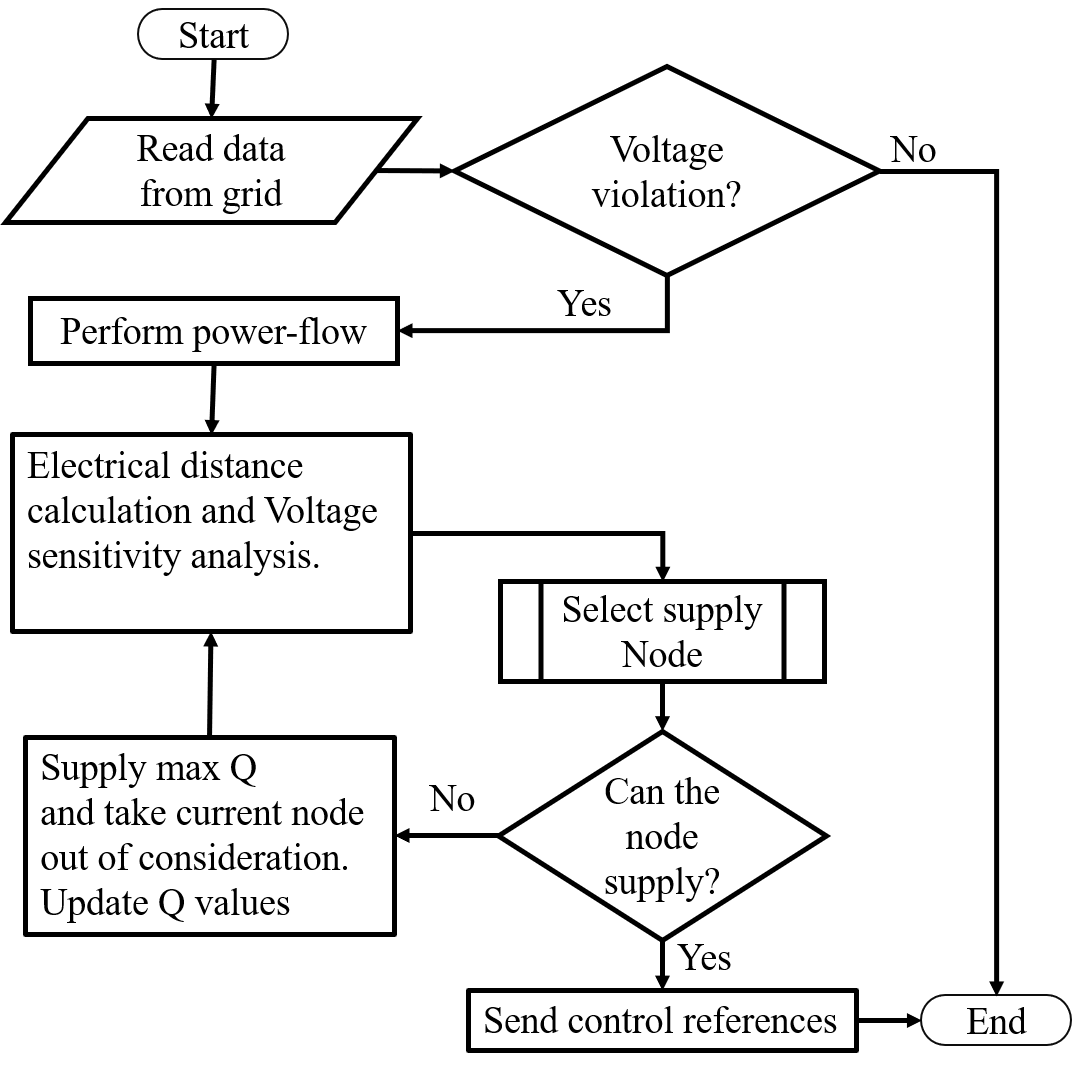
\includegraphics[width=0.8\linewidth]{figs/CVC_FLOWCHART_NEW.png}
\caption{Flowchart of the proposed CVC scheme}
\label{fig:Overview}
\end{figure}

\begin{figure}[!h]
\centering
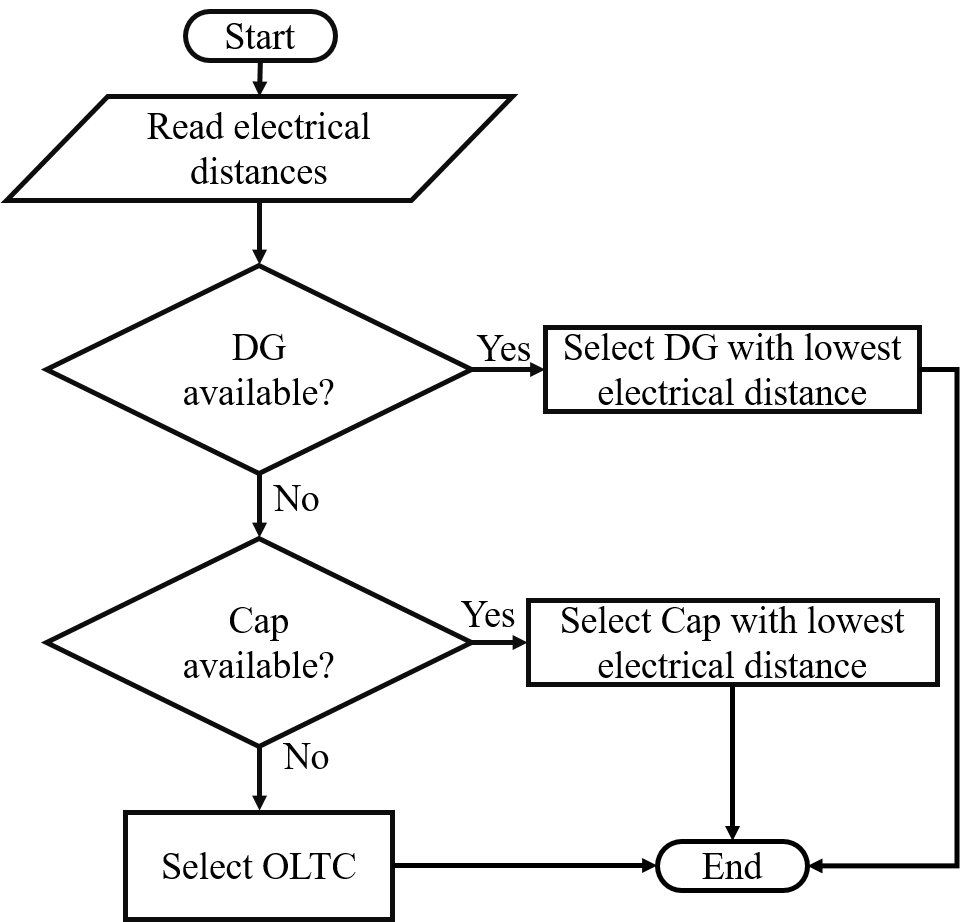
\includegraphics[width=0.8\linewidth]{figs/Flow_chart_2_1.png}
\caption{Flow chart of the 'Select supply node' subroutine}
\label{fig:sub_rou}
\end{figure}

\begin{enumerate}
    \item \textbf{Voltage violation?:} At the start of the algorithm it checks for a signal from the distribution system to see if a violation has occurred. It is assumed that the distribution system has systems in place to detect voltage violations as the purpose of the algorithm is to coordinate the response of the available resources to mitigate the violation. If there is no violation detected the algorithm does not take any actions. If a violation has occurred the algorithm continues.
    
    \item \textbf{Read data from grid:} In this step the algorithm reads the real power $P$ and reactive power $Q$ demands from all the loads and inverter interfaced DGs in the system. It also receives the status of the capacitor banks (ON/OFF) and the current tap position of any on load tap changer (OLTC) available in the system. And finally, it receives voltage magnitude $|V|$ measurements from any points of the system where such measurements are available.
    
    % The distribution grid block represents the actual distribution grid the proposed CVC will be in charge of. The distribution grid will provide the real and reactive power P and Q and the voltage magnitude $|V|$ of all the measured points from the system to the algorithm when a voltage violation is detected.
    % \item \textbf{Bad data detection:} This section will make use of bad data detection algorithms to determine bad data received from the system. This step will filter out the bad data and provide the next step with accurate system data. (This will be the last step developed and might not be included in the IET special issue paper planned to be submitted at FALL 2019).
    \item \textbf{Perform power-flow:} In this step, the algorithm performs power-flow using the data acquired in the previous step to estimate the remaining voltage angles and magnitudes of nodes that do not have measurements. 
    
    \item \textbf{Voltage sensitivity analysis and electrical distance calculation:} Using the data from the power-flow in this step, the voltage sensitivity analysis, and electrical distance calculations will be performed to determine the best node to supply reactive power compensation to aid in voltage regulation. This step also determines how much reactive power compensation should the selected node provide. These concepts have been explained in detail in Section \ref{vsa} and \ref{edc}.
    
    \item \textbf{Select supply node:} This subroutine is shown in Fig. \ref{fig:sub_rou}. The subroutine starts by reading the electrical distances from the previous steps. Then it first checks to see if there are any DGs available to supply reactive power in the 'DG available?' step. If there are it selects the DG with the least electrical distance to supply reactive power compensation. Otherwise, it checks for capacitor banks available if the 'Cap available?' step. If there are capacitor banks available to be turned on or off to tackle the voltage violation the subroutine selects the capacitor bank with the lowest electrical distance. Finally, if there are no DG or capacitor banks available, OLTC is selected to mitigate the voltage violation. 
    
    \item \textbf{Can the node supply?:} This step checks if the resources available at the selected node has the capability to supply the required reactive power compensation. If it does, the algorithm moves on to the 'Send Q references' step. Otherwise, it goes to the 'Supply max Q and takes current node out of consideration' step.
    
    %the reactive power reference is sent to the actual equipment available at the distribution grid. Otherwise, the algorithm updates the resources at the current node to supply maximum reactive power and sends the updated system status to Voltage sensitivity analysis and electrical distance calculation and the algorithm runs voltage sensitivity analysis and electrical distance calculation again to find the next best node to supply reactive power from. When a solution is reached the algorithm sends the Q references to the respective nodes
    
     \item \textbf{Supply max Q and take the current node out of consideration:} This step sets the current best node to supply the maximum Q possible and takes it out of the list of available nodes with reactive power resources. Then it sends the updated node status to the 'Voltage sensitivity analysis and electrical distance calculation' step to find the next best node to supply reactive power to mitigate the voltage violation.
     
     \item \textbf{Send Q references} In this step, the algorithm sends the updated Q references to all the nodes available in the system.
\end{enumerate}



\section{Offline validation}
\label{off1}
The SUNGRIN test feeder 2 \cite{SG} was used to validate the algorithm. The feeder is modeled using data collected from an actual distribution system based in Florida. The feeder consists of nine busses with three PV sights. The inverter interfaced PVs in the feeder are represented as controlled current sources in the offline simulation. The feeder was modeled and simulated in Simulink using the Simscape Power Systems\textsuperscript{TM} library in the phasor domain. The CVC algorithm was run as a Matlab function inside the Simulink simulation. Fig. \ref{fig:feeder2} show the one-line diagram of the feeder used in the offline validation.
\begin{figure}[!htb]
\centering
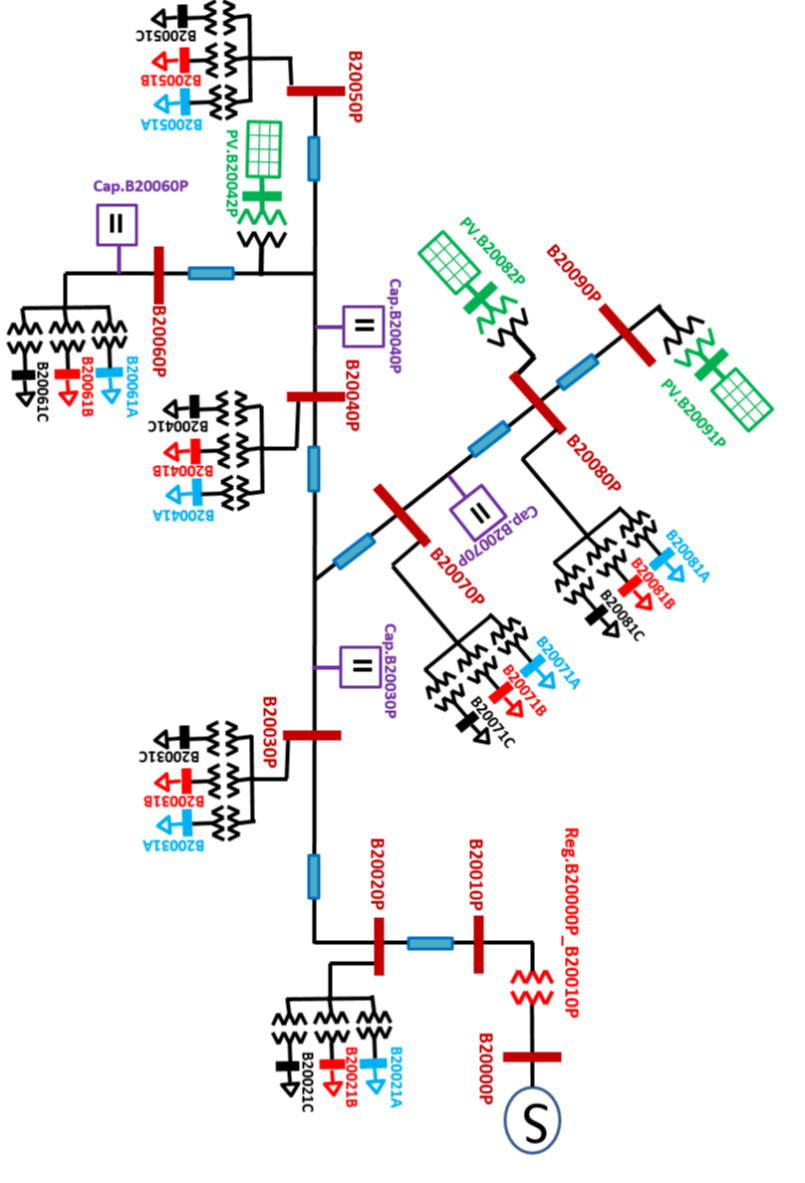
\includegraphics[width=0.9\linewidth]{figs/feeder_r.png} 
\caption{Distribution feeder used for validation}
\label{fig:feeder2}
\end{figure}

Fig. \ref{fig:without_vvc} shows the feeder voltage without coordinated voltage control during normal operation for one day. The dashed line on top represents the Upper limit (UL) for the voltage and the dashed line at the bottom represents the lower limit (LL) for the voltage. The upper and lower limits are set as 1.05 PU and 0.95 PU respectively. The solid lines represent voltages of busses B20010P to B20090P. They are labeled as V1 for bus B20010P, V2 bus for B20020P, V3 for bus B20030P and so on. As it can be seen in Fig. \ref{fig:without_vvc} the voltage profiles go above 1.06 PU and as low as 0.92 PU during regular operations during the 24-hour run. 
Fig. \ref{fig:with_cvc} shows the feeder voltages with coordinated voltage control implemented. It can be seen that the coordinated voltage control scheme is able to maintain the voltages within the UL and LL. This is possible by coordinating the use of the reactive power generation capabilities of the DG inverters with the traditional regulation devices. The reactive power supplied by the DG inverters are shown in Fig. \ref{fig:DG_Q}. Here QPV1, QPV2, and QPV3 represent the reactive power supplied by the inverter interfaced PVs located at bus B20040P, B20080P, and B20090P respectively. It can be observed that the DG interfaced inverters provide proper positive and negative reactive power compensation to compensate for voltage violation. The capacitor bank operations are shown in Fig. \ref{fig:cap_bank}. Here CAP1, CAP2, and CAP3 represent the capacitor banks located at bus B20040P, B20030P and B20070P respectively. The capacitor bank located at bus B20060P is defined as always on in the circuit configuration. So it is not considered in the control scheme. It can be observed in Fig. \ref{fig:cap_bank} that the capacitor banks closest to the nodes with voltage violation (CAP1 and CAP3) are being turned off during upper limit violation and during the lower limit violation CAP3 in being turned back on to deal with the lower limit violation. It should be noted there was no need for an OLTC operation to mitigate the voltage violation. This shows that with proper coordination of available resources the operation of mechanical regulation devices can be minimized increasing their life span and reducing the cost of operation. In the offline simulation, the CVC algorithm was fed the real, reactive power data as well as the voltage and current magnitude and angle data from all the nodes directly from the simulation. So the power-flow step shown in Fig. \ref{fig:Overview} was skipped in the off-line implementation as all the required data were considered to be available directly from the system. Also, the algorithm was executed for every simulation step synchronously with the power system simulation. This simulation was performed as an initial validation of the CVC algorithm for rapid prototyping. To see the behavior of the CVC algorithm in a more practical scenario real-time validation was performed.

\begin{figure}[!htb]
\centering
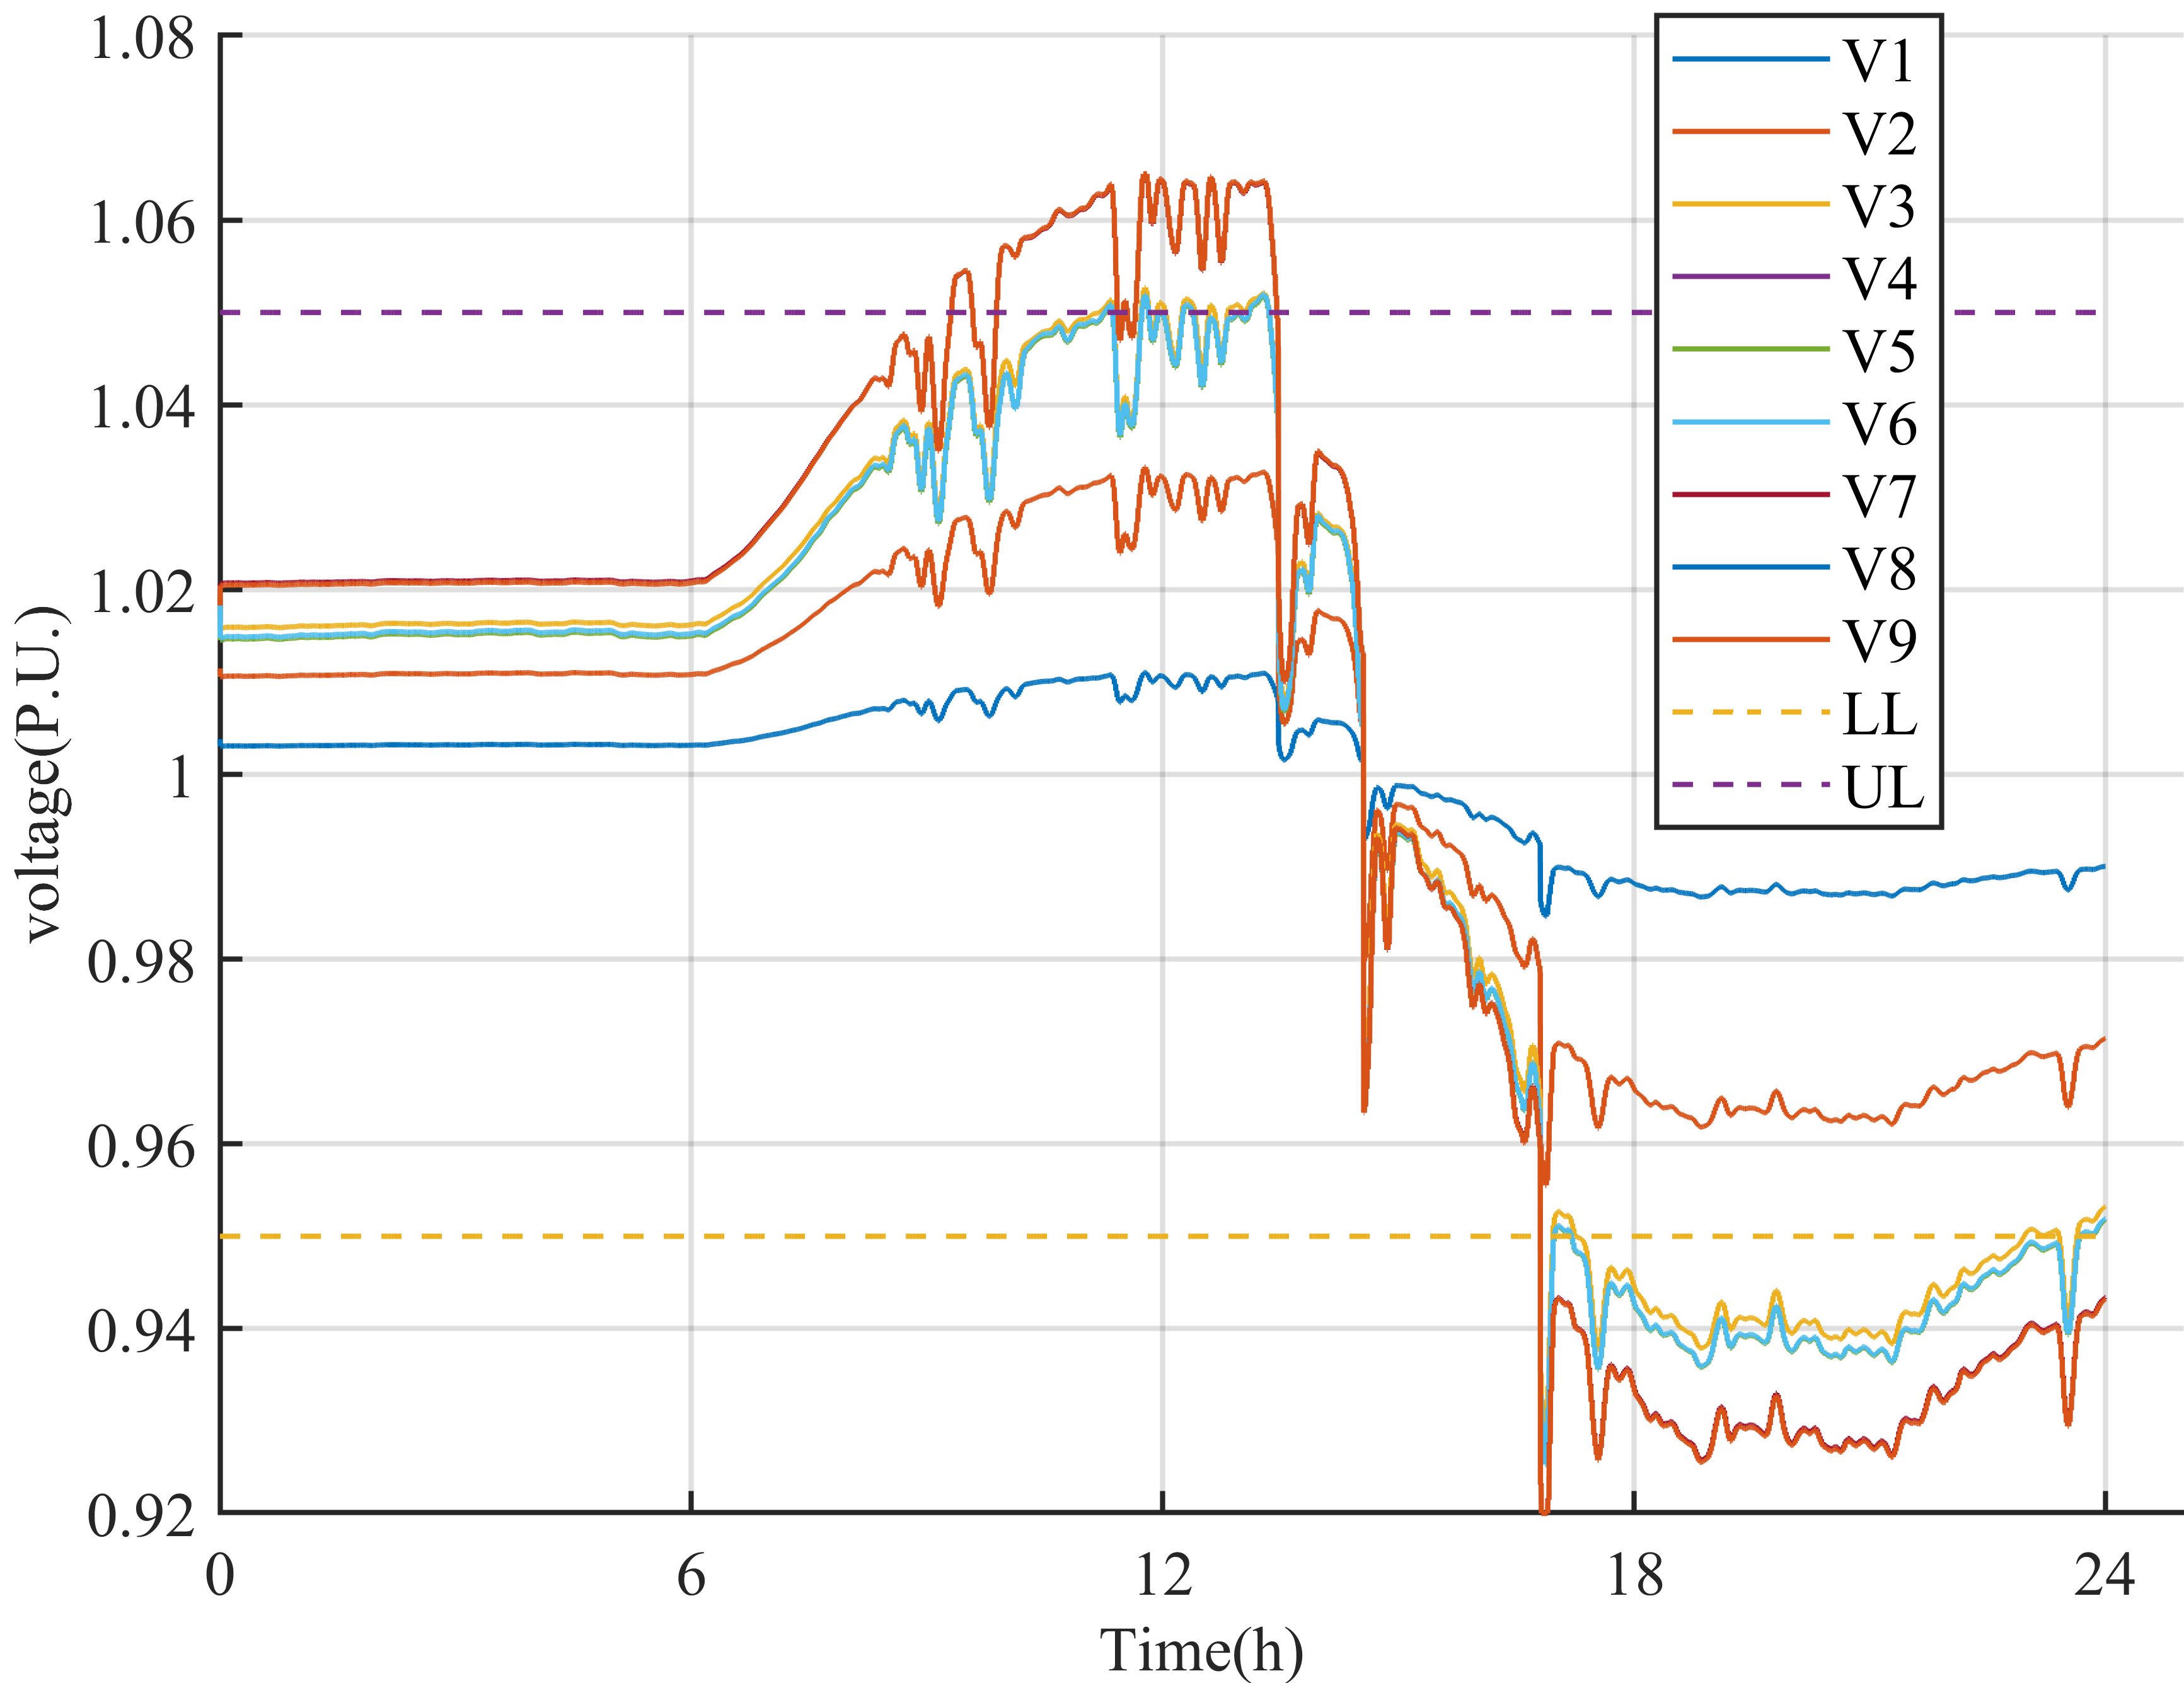
\includegraphics[width=\linewidth]{figs/NEW_WITHOUT_VVC.png}
\caption{Voltage Profile without Coordinated Voltage Control}
\label{fig:without_vvc}
\end{figure}

\begin{figure}[!htb]
\centering
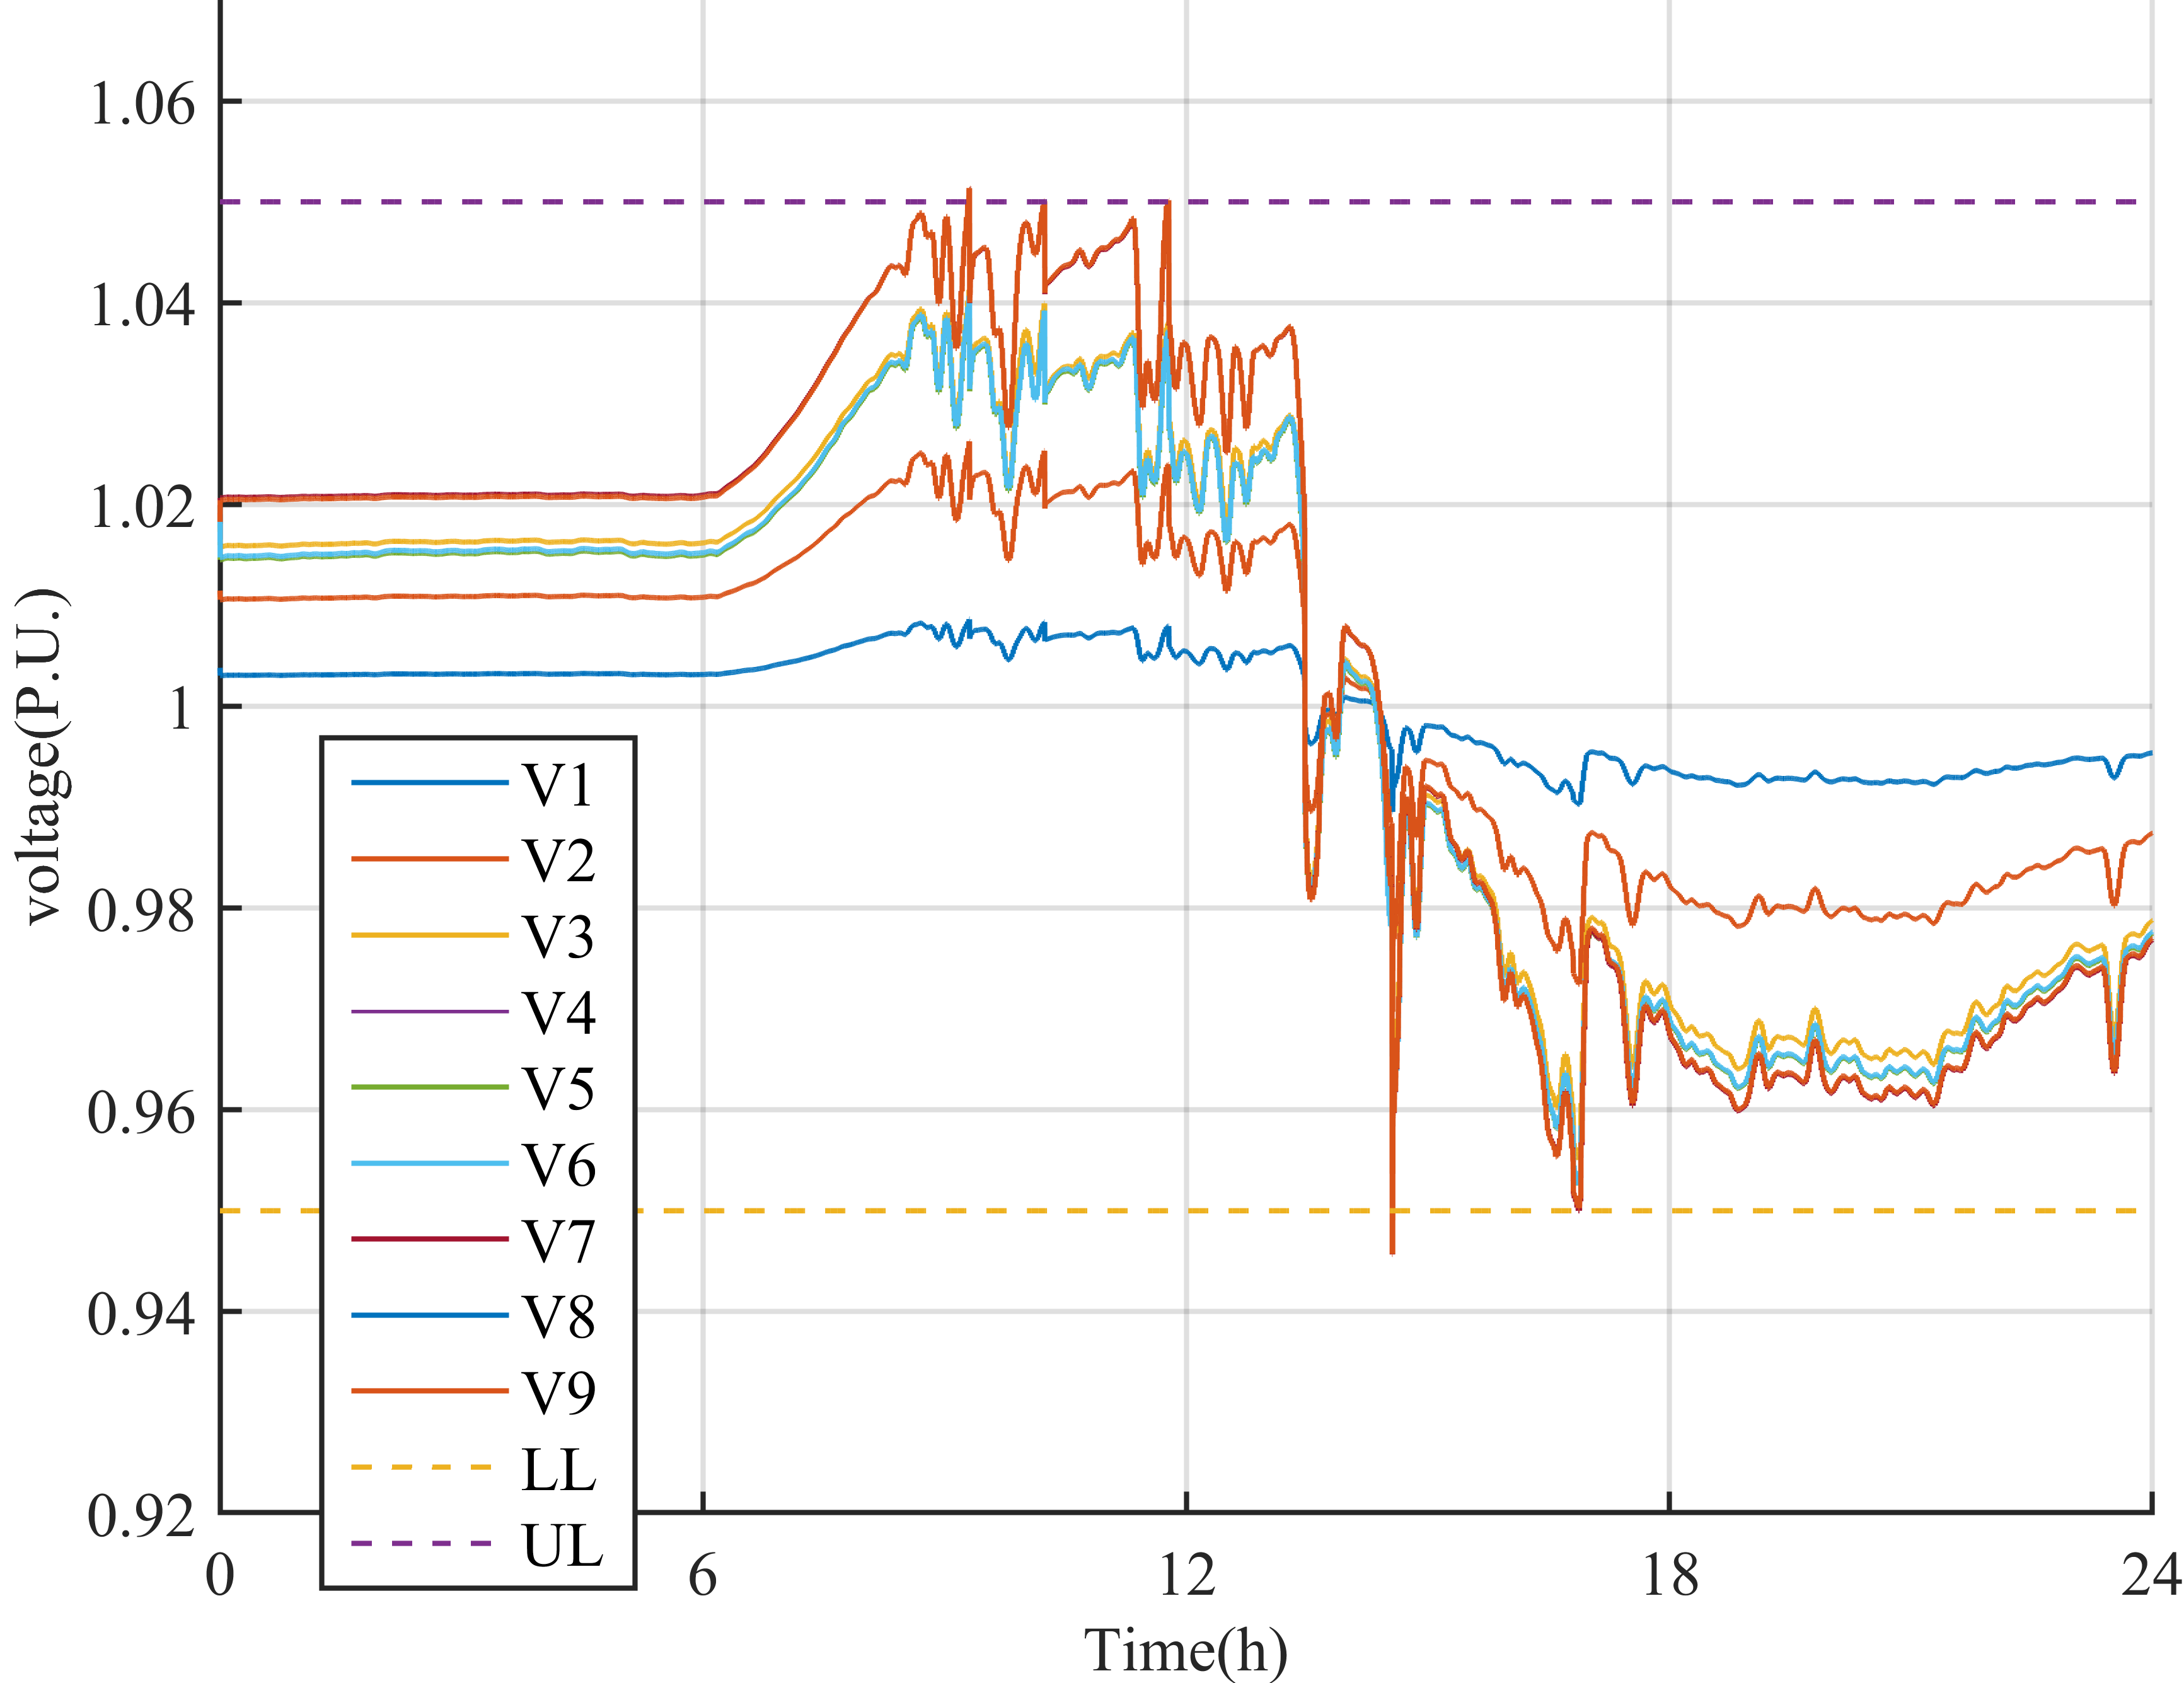
\includegraphics[width=\linewidth]{figs/NEW_WITH_VVC.png}
\caption{Voltage profile with coordinated voltage control}
\label{fig:with_cvc}
\end{figure}


\begin{figure}[!htb]
\centering
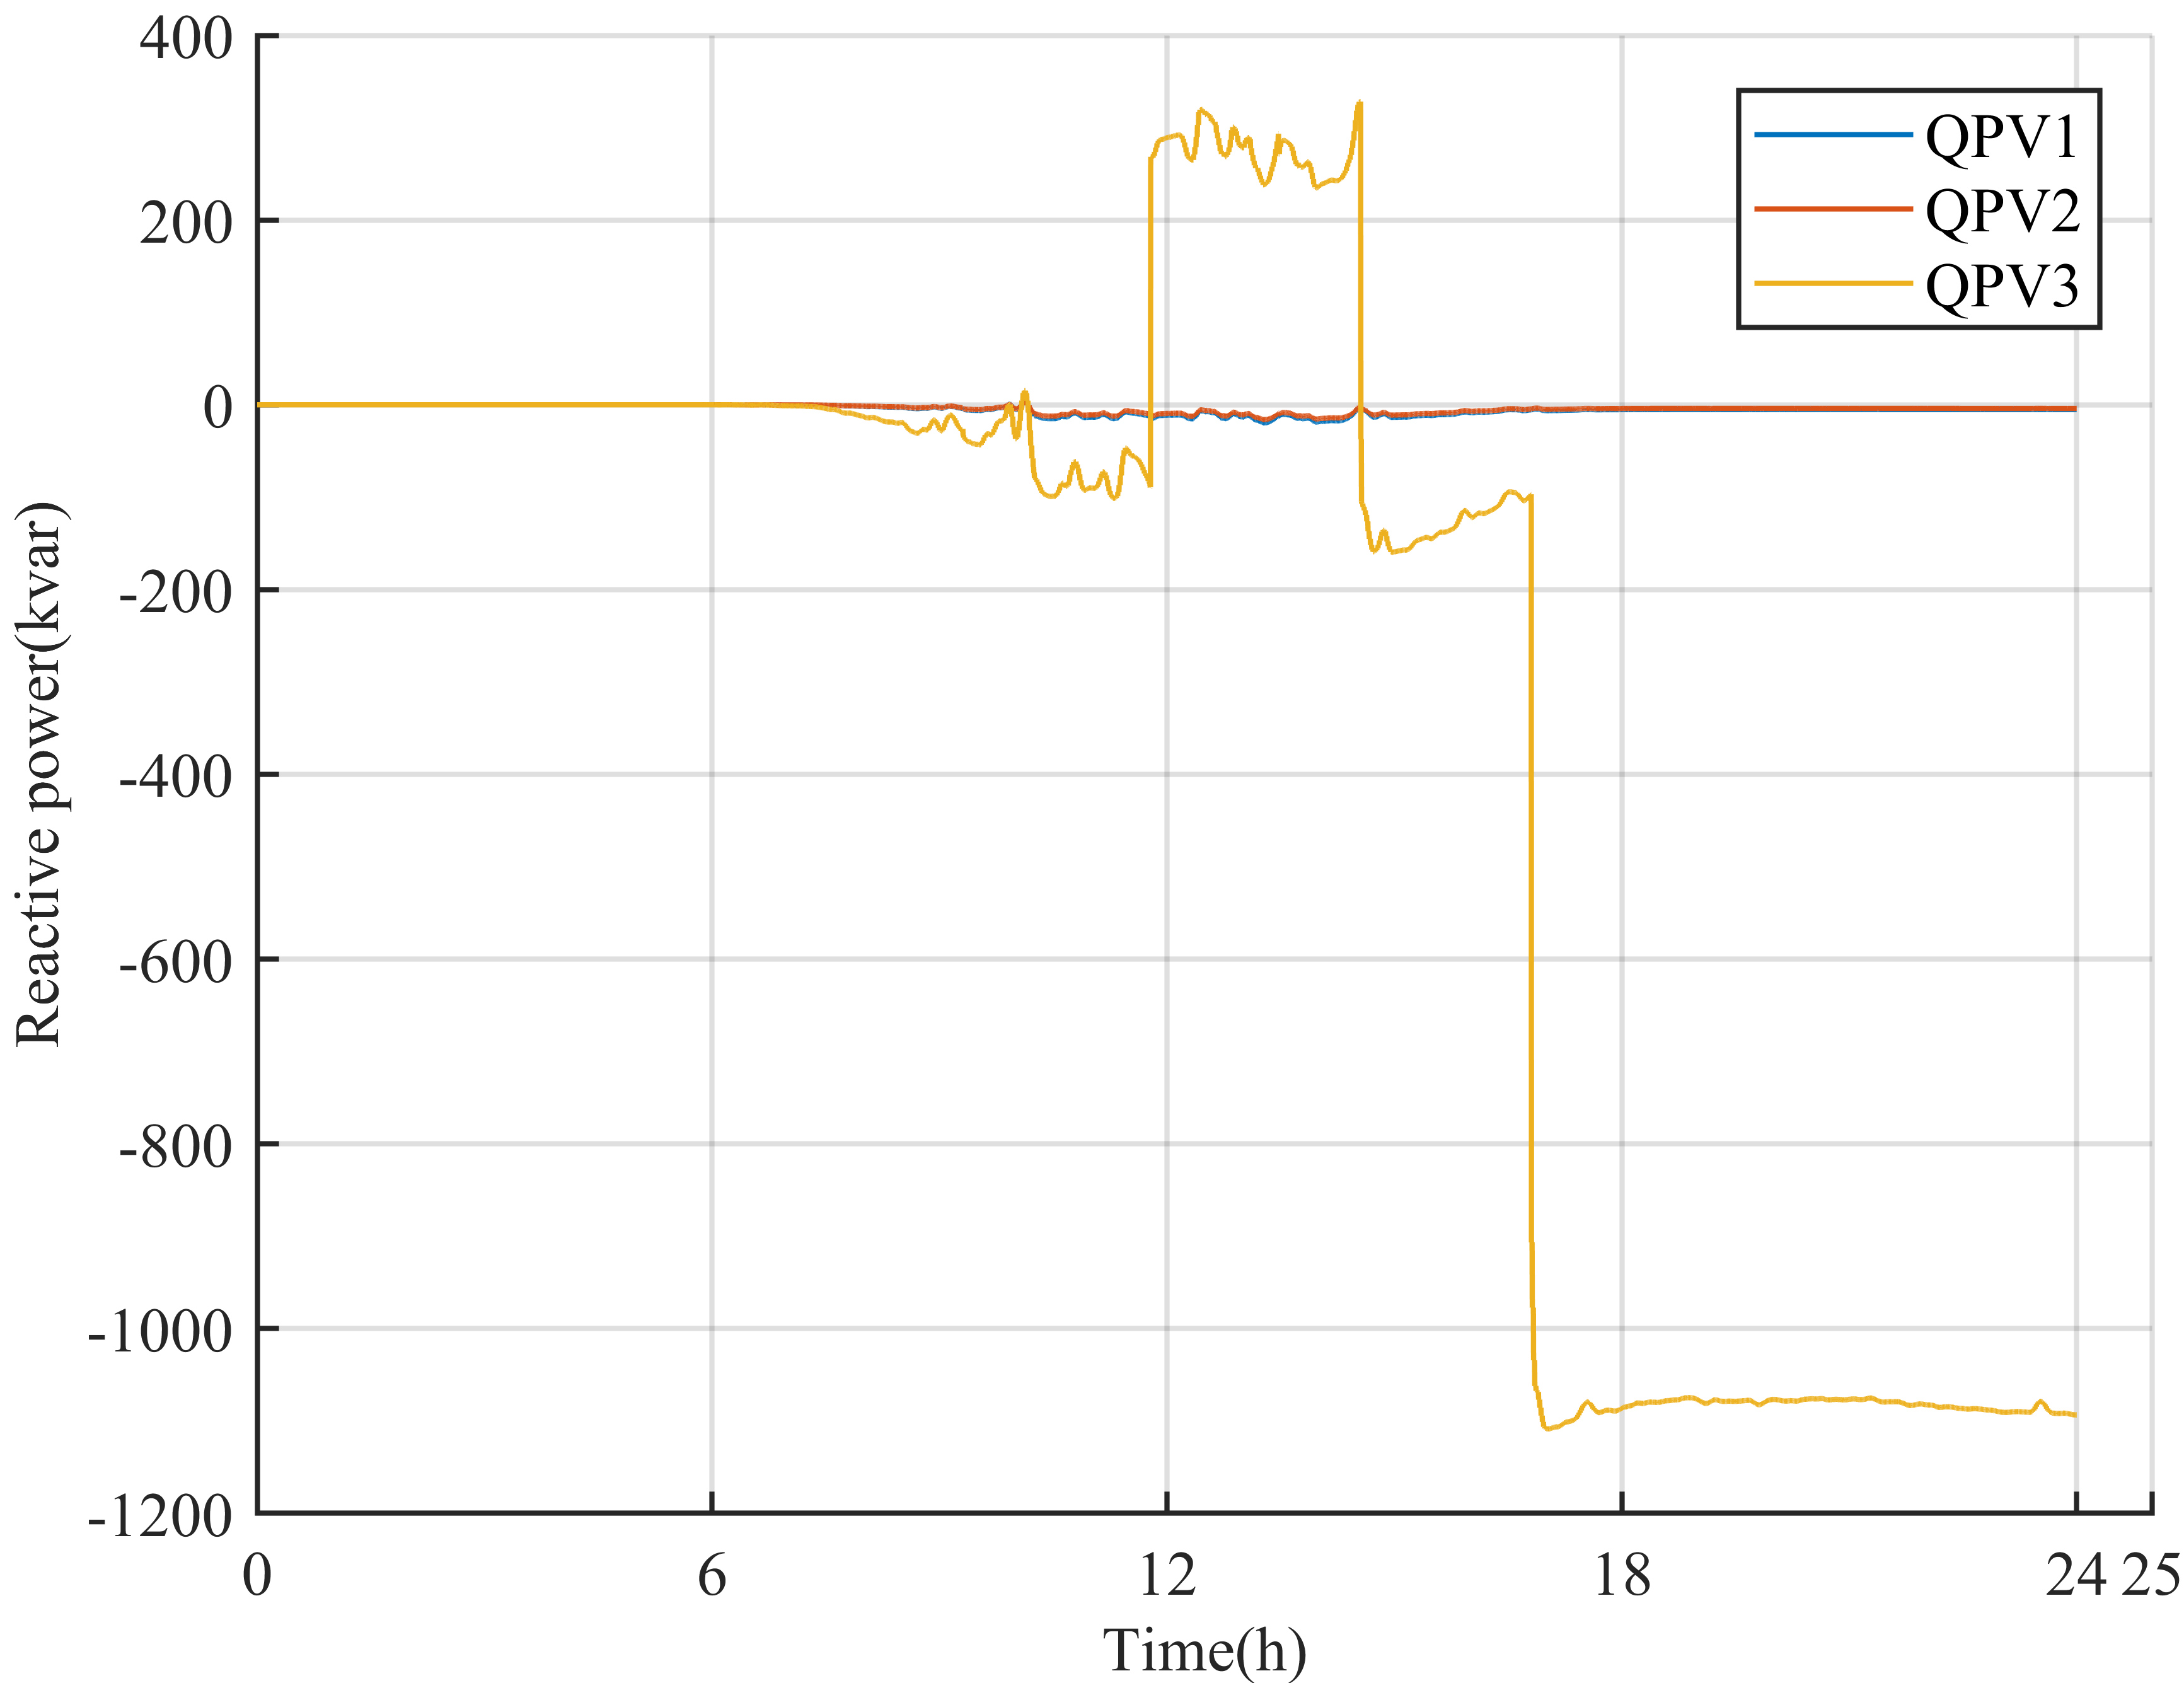
\includegraphics[width=\linewidth]{figs/NEW_PQ.png}
\caption{Reactive power supplied by DGs}
\label{fig:DG_Q}
\end{figure}

\begin{figure}[!htb]
\centering
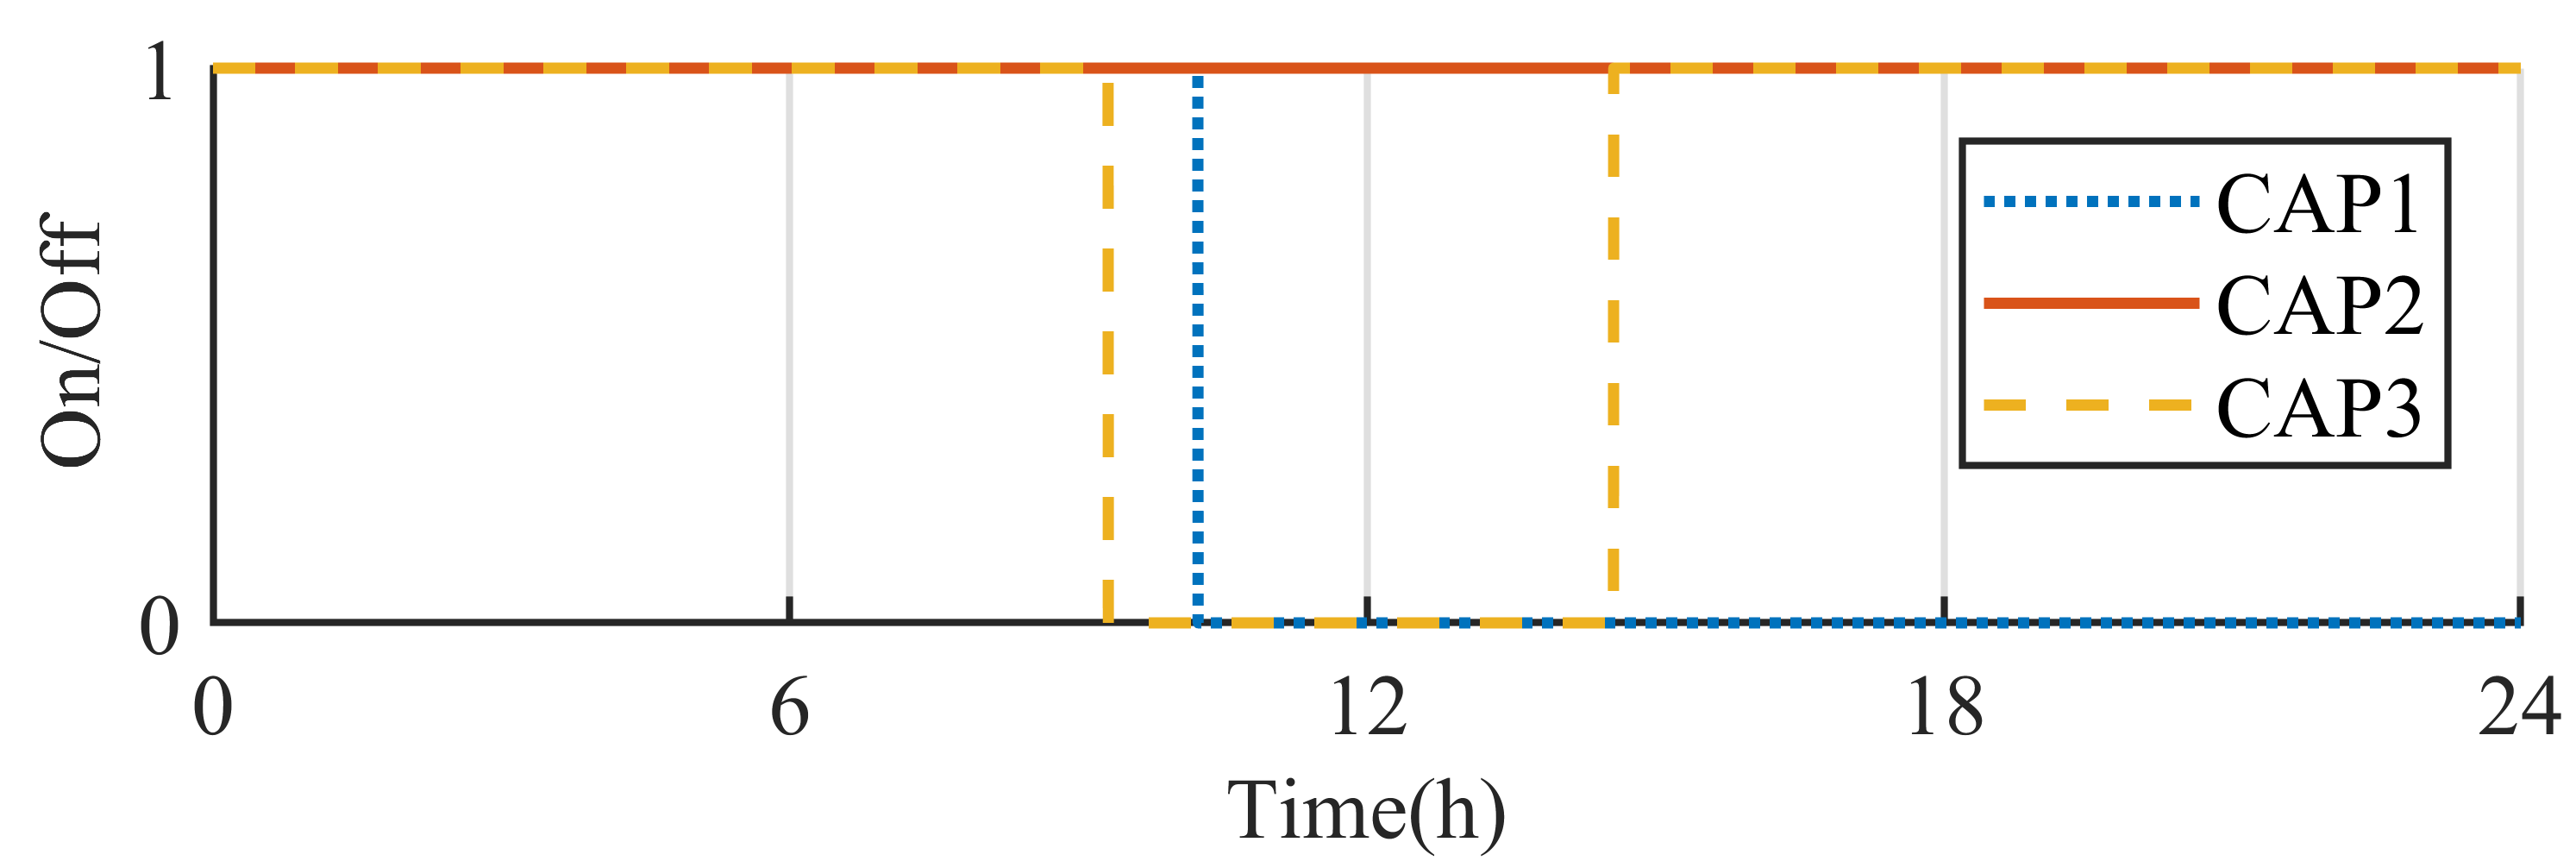
\includegraphics[width=\linewidth]{figs/NEW_CAPS.png}
\caption{Capacitor bank switching states}
\label{fig:cap_bank}
\end{figure}

\section{Controller hardware in the loop validation}\label{chil}
\subsection{Overview of the testbed}
Although the algorithm performed well in the offline simulation, it is not enough just to validate the algorithm in an off-line environment. To validate the feasibility of the algorithm for practical use real-time controller hardware in the loop (CHIL) simulation was performed. The CHIL testbed and python API presented in \cite{newaz2019controller} was used for the CHIL validation of the CVC algorithm. Fig. \ref{fig:CHIL_BLOCK} represents the block diagram of the CHIL setup. In the case of the real-time CHIL simulation, a more realistic scenario was considered. It was considered that the real and reactive power information from the load points and the inverters were available. Also, the current status of the capacitor banks and OLTC was available. Finally, voltage violation detection signal as well as the current voltage magnitude and voltage angle at the substation was available. Besides that, no other information was available from the system. The actual CHIL setup is shown in Fig. \ref{fig:CHIL_SETUP}. The CHIL simulation setup consists of three major components.

\begin{figure*}[!h]
\centering
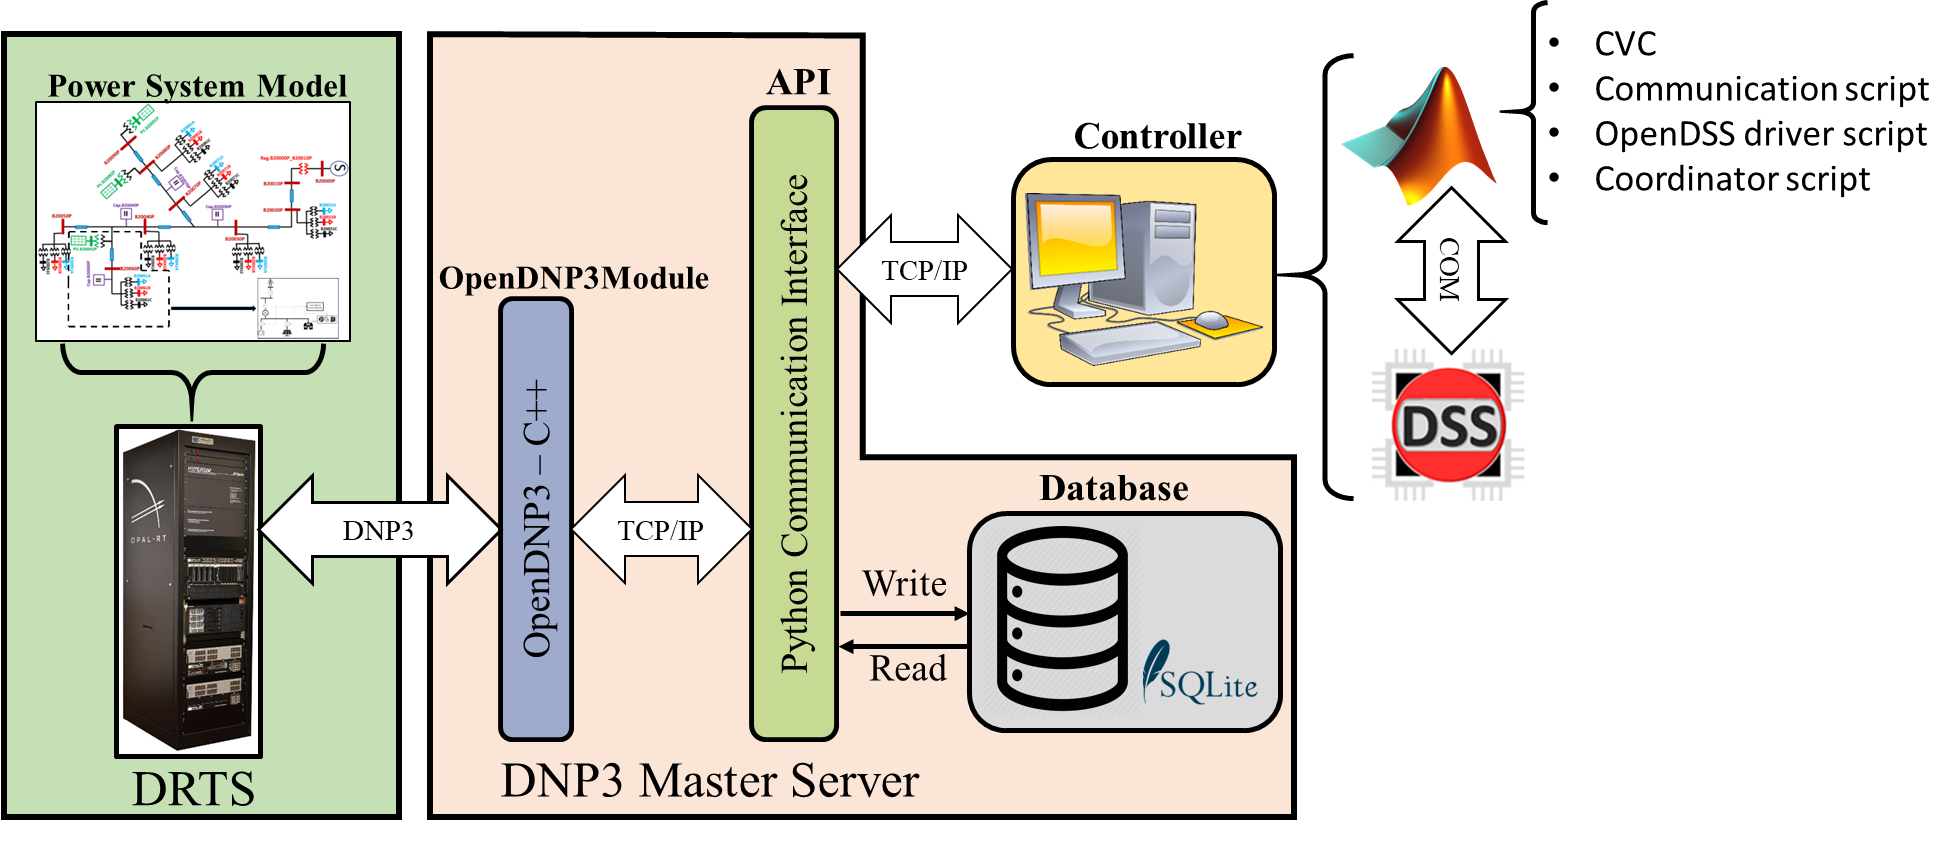
\includegraphics[width=\linewidth]{figs/RT_BLOCK_2.png}
\caption{CHIL block diagram}
\label{fig:CHIL_BLOCK}
\end{figure*}


\begin{figure}[!h]
\centering
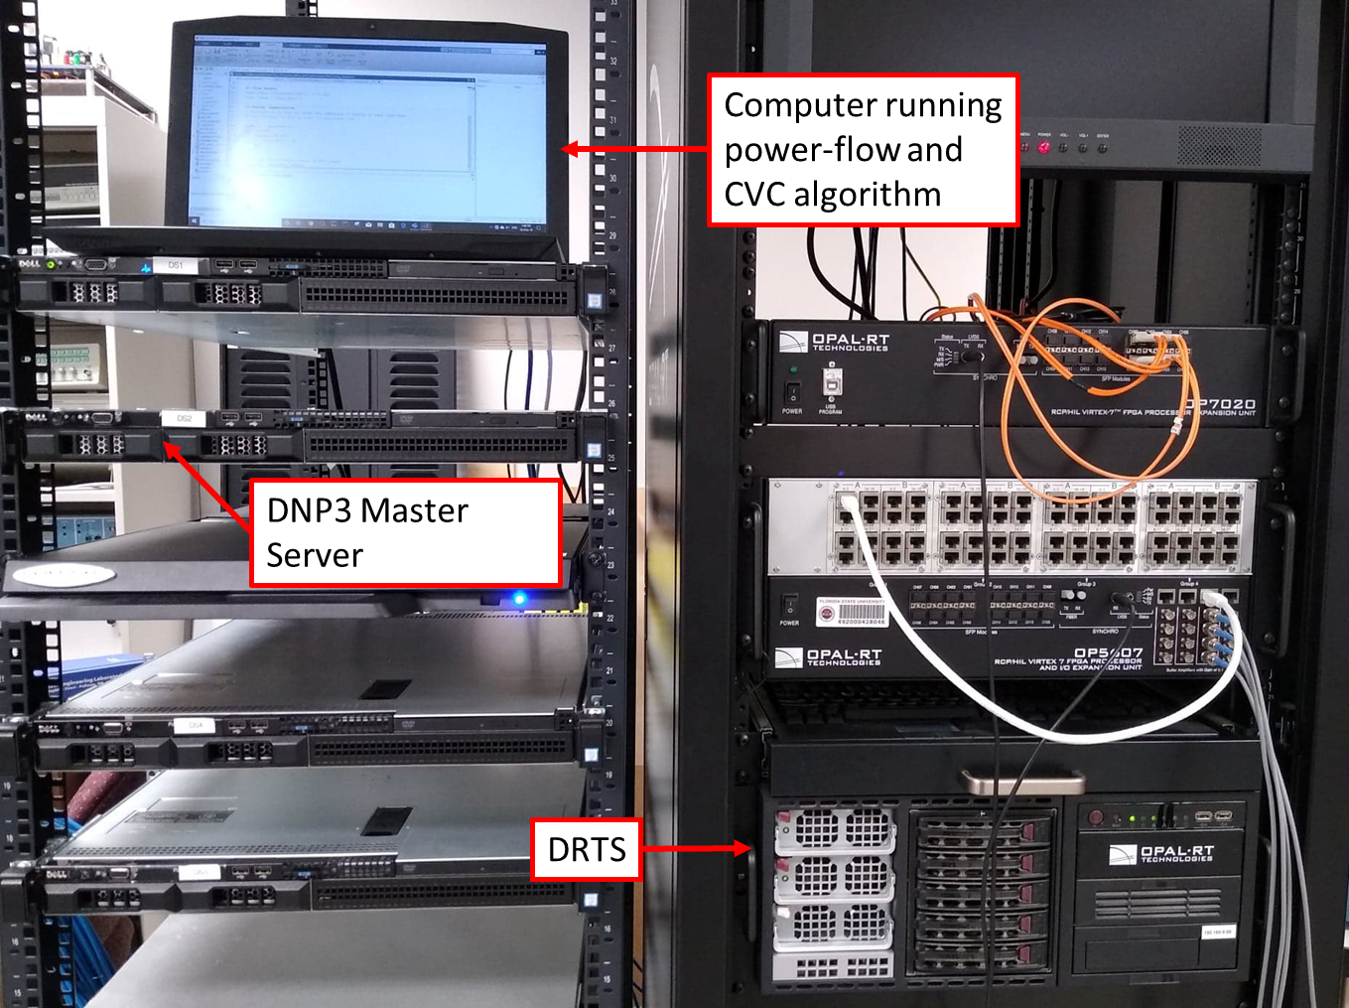
\includegraphics[width=\linewidth]{figs/LAB_SETUP.png}
\caption{Actual CHIL setup}
\label{fig:CHIL_SETUP}
\end{figure}


\subsubsection{Power System Modeled in Digital Real-time Simulator (DRTS}
It consists of different models designed to represent and simulate the behavior and interactions of grid-connected distributed energy resources (DERs) in a real-time environment. Some of these components are a) models of DERs (Lithium-ion batteries as energy storage systems (ES), Photovoltaic (PV) systems), b) dynamic load models designed to simulate dynamic loading conditions,  c) models of the distribution network and d) models of smart-meter devices designed to measure and communicate data such as voltages, currents, active power, and reactive power to the main (external) control system. All of these systems are modeled inside the digital real-time simulator (DRTS). 

\subsubsection{DNP3 Master Server}
The 'DNP3 Master Server' is in charge of sending and receiving data from the DRTS over DNP3. It also records the data and establishes connections with controllers.  It has the following main parts.
\begin{itemize}
    \item \textbf{OpenDNP3 C++} It consists of a real-world DNP3 communication infrastructure based on the OpenDNP3 \cite{opendnp3_2020} project. It communicates with the smart-meter models inside the DRTS via the IEEE 1815 DNP3 communication protocol. It also sends data back to the DRTS using DNP3 as well. It is programmed in C++ using OpenDNP3 as a base to enable DNP3 communication.
    \item \textbf{Python Communication Interface:} This consists of application programming interfaces (APIs) designed to provide inter-process communication to any generic control algorithm. They provide a communication bridge between the DNP3 communication module, a database management server, and any generic control algorithm devised to be deployed (and tested) in real-time system environments. The API is designed to work with SQL light databases. The API also allows any generic controller to send data to the communication layer to be sent to the DRTS.
    \item \textbf{Database} The database is there to store the data received over the DNP3 communication layer from the DRTS. In this implementation, an SQL light database was used. The 'Python Communication Interface' layer writes the data received over DNP3 in the database it also enables sending of the data to the outside control algorithm.
\end{itemize}

\subsubsection{Controller:}
The controller, in this case, is a computer running the power-flow and CVC algorithm. The CVC algorithm and power-flow are controlled using a coordinator script. This is a script written in the Matlab scripting language to communicate with the Controller-to-database API over TCP/IP and execute the various sections of the CVC algorithm in proper order. The coordinator script starts by running the communication script to receive the reinvent data from the DNP3 Master Server. Then it runs a power-flow using openDSS based on the current data. This is done by configuring and controlling the openDSS engine oven the windows COM interface. After running the power-flow the the coordinator script runs the CVC algorithm to get the reactive power compensation needed. And then it runs the communication script again to send the control actions back to the DNP3 Master Server over TCP/IP and the DNP3 Master Server relays the data to the DRTS simulation over DNP3.
% over the API shown in Fig.\ref{fig:Overview} and sends it to the power-flow step. The power-flow is performed using openDSS. An openDSS model of the feeder shown in Fig. \ref{fig:feeder2} is modeled in open DSS and the power-flow step changes the power values of all the loads and sources according to the data received from the real-time simulation. Then the system is solved to get the P, Q,|V| and $\delta$ data as seen in Fig. \ref{fig:Overview}. The master script then uses this data to run the Electrical distance calculations and voltage sensitivity analysis and follows the process discussed in chapter \ref{CVC} until it reaches the Send Q references step. Then it sends the required Q references to the Controller-to-database API over TCP/IP and the API relays the data to the DRTS through the communication layer of the database manager.

\subsection{Real-time CHIL results}
The real-time simulation was run for 900 seconds using the system PV and load profile used in the offline simulation. The simulation uses the system profile between 38160s to 39060s. Fig. \ref{fig:RT_VVC} shows the whole real-time simulation voltage profiles. The dashed line represents the upper limit 'UL' of the voltage bounds. The rest of the legend uses the same notations as Fig.\ref{fig:with_cvc}. It can be seen in the figure that the real-time implementation of the algorithm is able to mitigate the voltage violation that occurs during the simulation. Fig. \ref{fig:RT_VS_OFF_V} shows the voltage profile of 'V7' for both the offline and real-time simulation. The solid line represents the offline and the dotted line represents the real-time profile. It can be seen that the real-time simulation takes 11s to mitigate the voltage violation where the offline simulation took 2s. This is expected as the real-time simulation implements a real-world communication infrastructure with smart meters and a power-flow step to estimate the system status. This response time is comparable to the current voltage regulation schemes which take around 5s to 10s to coordinate system voltages. Other than that the offline and real-time profiles deviate less than 2\%. 'V7' is chosen to be shown here because it shows the highest violation in the system. 

\begin{figure}[!h]
\centering
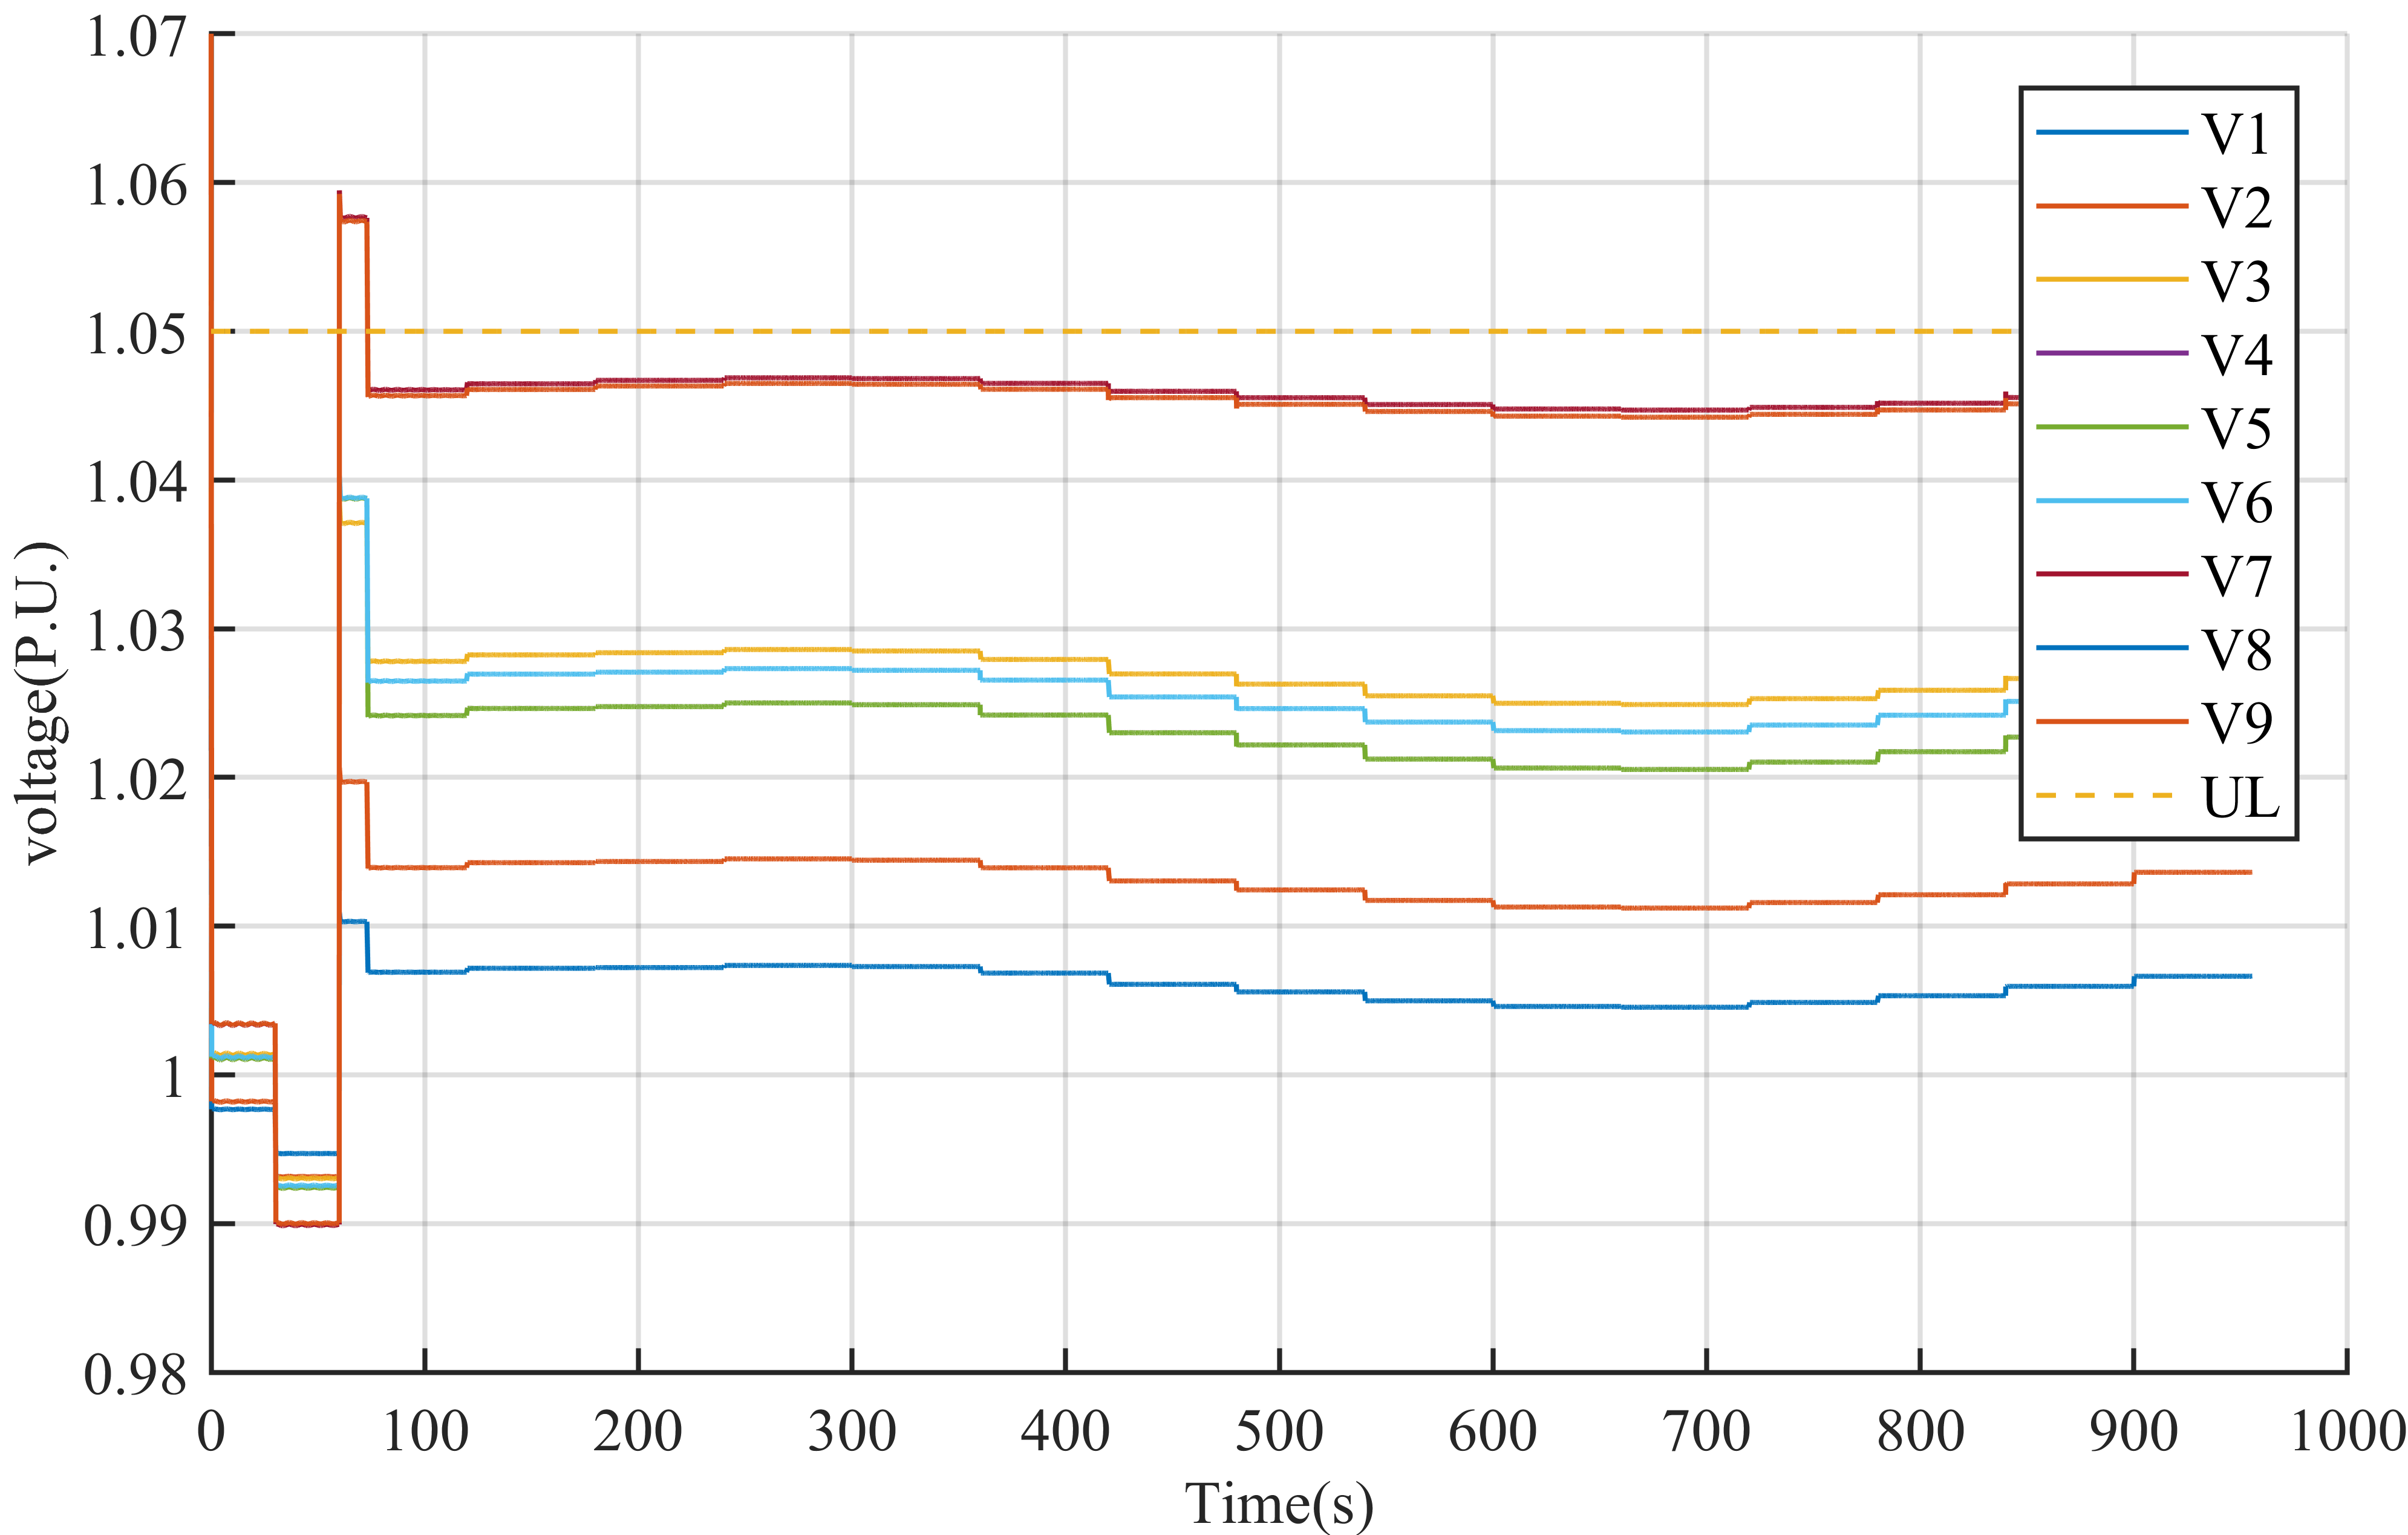
\includegraphics[width=\linewidth]{figs/RT_VOLTAGES.png}
\caption{Real-time voltage profile with coordinated voltage control.}
\label{fig:RT_VVC}
\end{figure}
% As the beginning of the 24-hour profile did not have any voltage violations the real-time simulation was run from 9:00 AM to 12:00 AM. This was done to save time and resources used for real-time validation. Fig. \ref{fig:RT_VVC} shows the voltage profile of the system for real-time simulation with CVC active. It should be noted that the same load and DG profiles were used for off-line and real-time validation. It can be observed that the voltage profile of the system is within the upper and lower limit. Fig. \ref{fig:RT_VVC} uses the same notation as Fig. \ref{fig:with_cvc}. The voltage profiles are a lot more fluctuations compared to the off-line simulation in this case. This is due to the fact that unlike the offline validation the CVC algorithm is not running synchronously with the real-time simulation. This causes a delay in communication and response time and the algorithm does not have the most recent state of the system. So the algorithm receives data from a few seconds back and does not immediately see the effects of its actions. This causes the algorithm to provide extra commands to the DG inverts. This can be seen more clearly in Fig. \ref{fig:RT_PQ}. It can be seen that the references to the DG inverters are a lot more varied in this case compared to the off-line validation. The algorithm behaves differently while compensating for the under-voltage case as well. As it can be seen in Fig \ref{fig:RT_CAP}, instead of using the DG inverters the algorithm decided to use the CAP1 capacitor bank in this case. In the offline simulation, the algorithm used the DG inverters to compensate instead. Although the algorithm behaves differently in the real-time simulation it is still able to maintain the system voltage within the upper and lower limits. The maximum round trip communication time seen in the real-time implementation was 12 seconds. Another reason for the different behavior might be due to the power-flow step. As mentioned before, the offline simulation uses the actual states of the system for all it's calculations but the real-time CHIL simulation uses estimated states based on a power-flow.

\begin{figure}[!h]
\centering
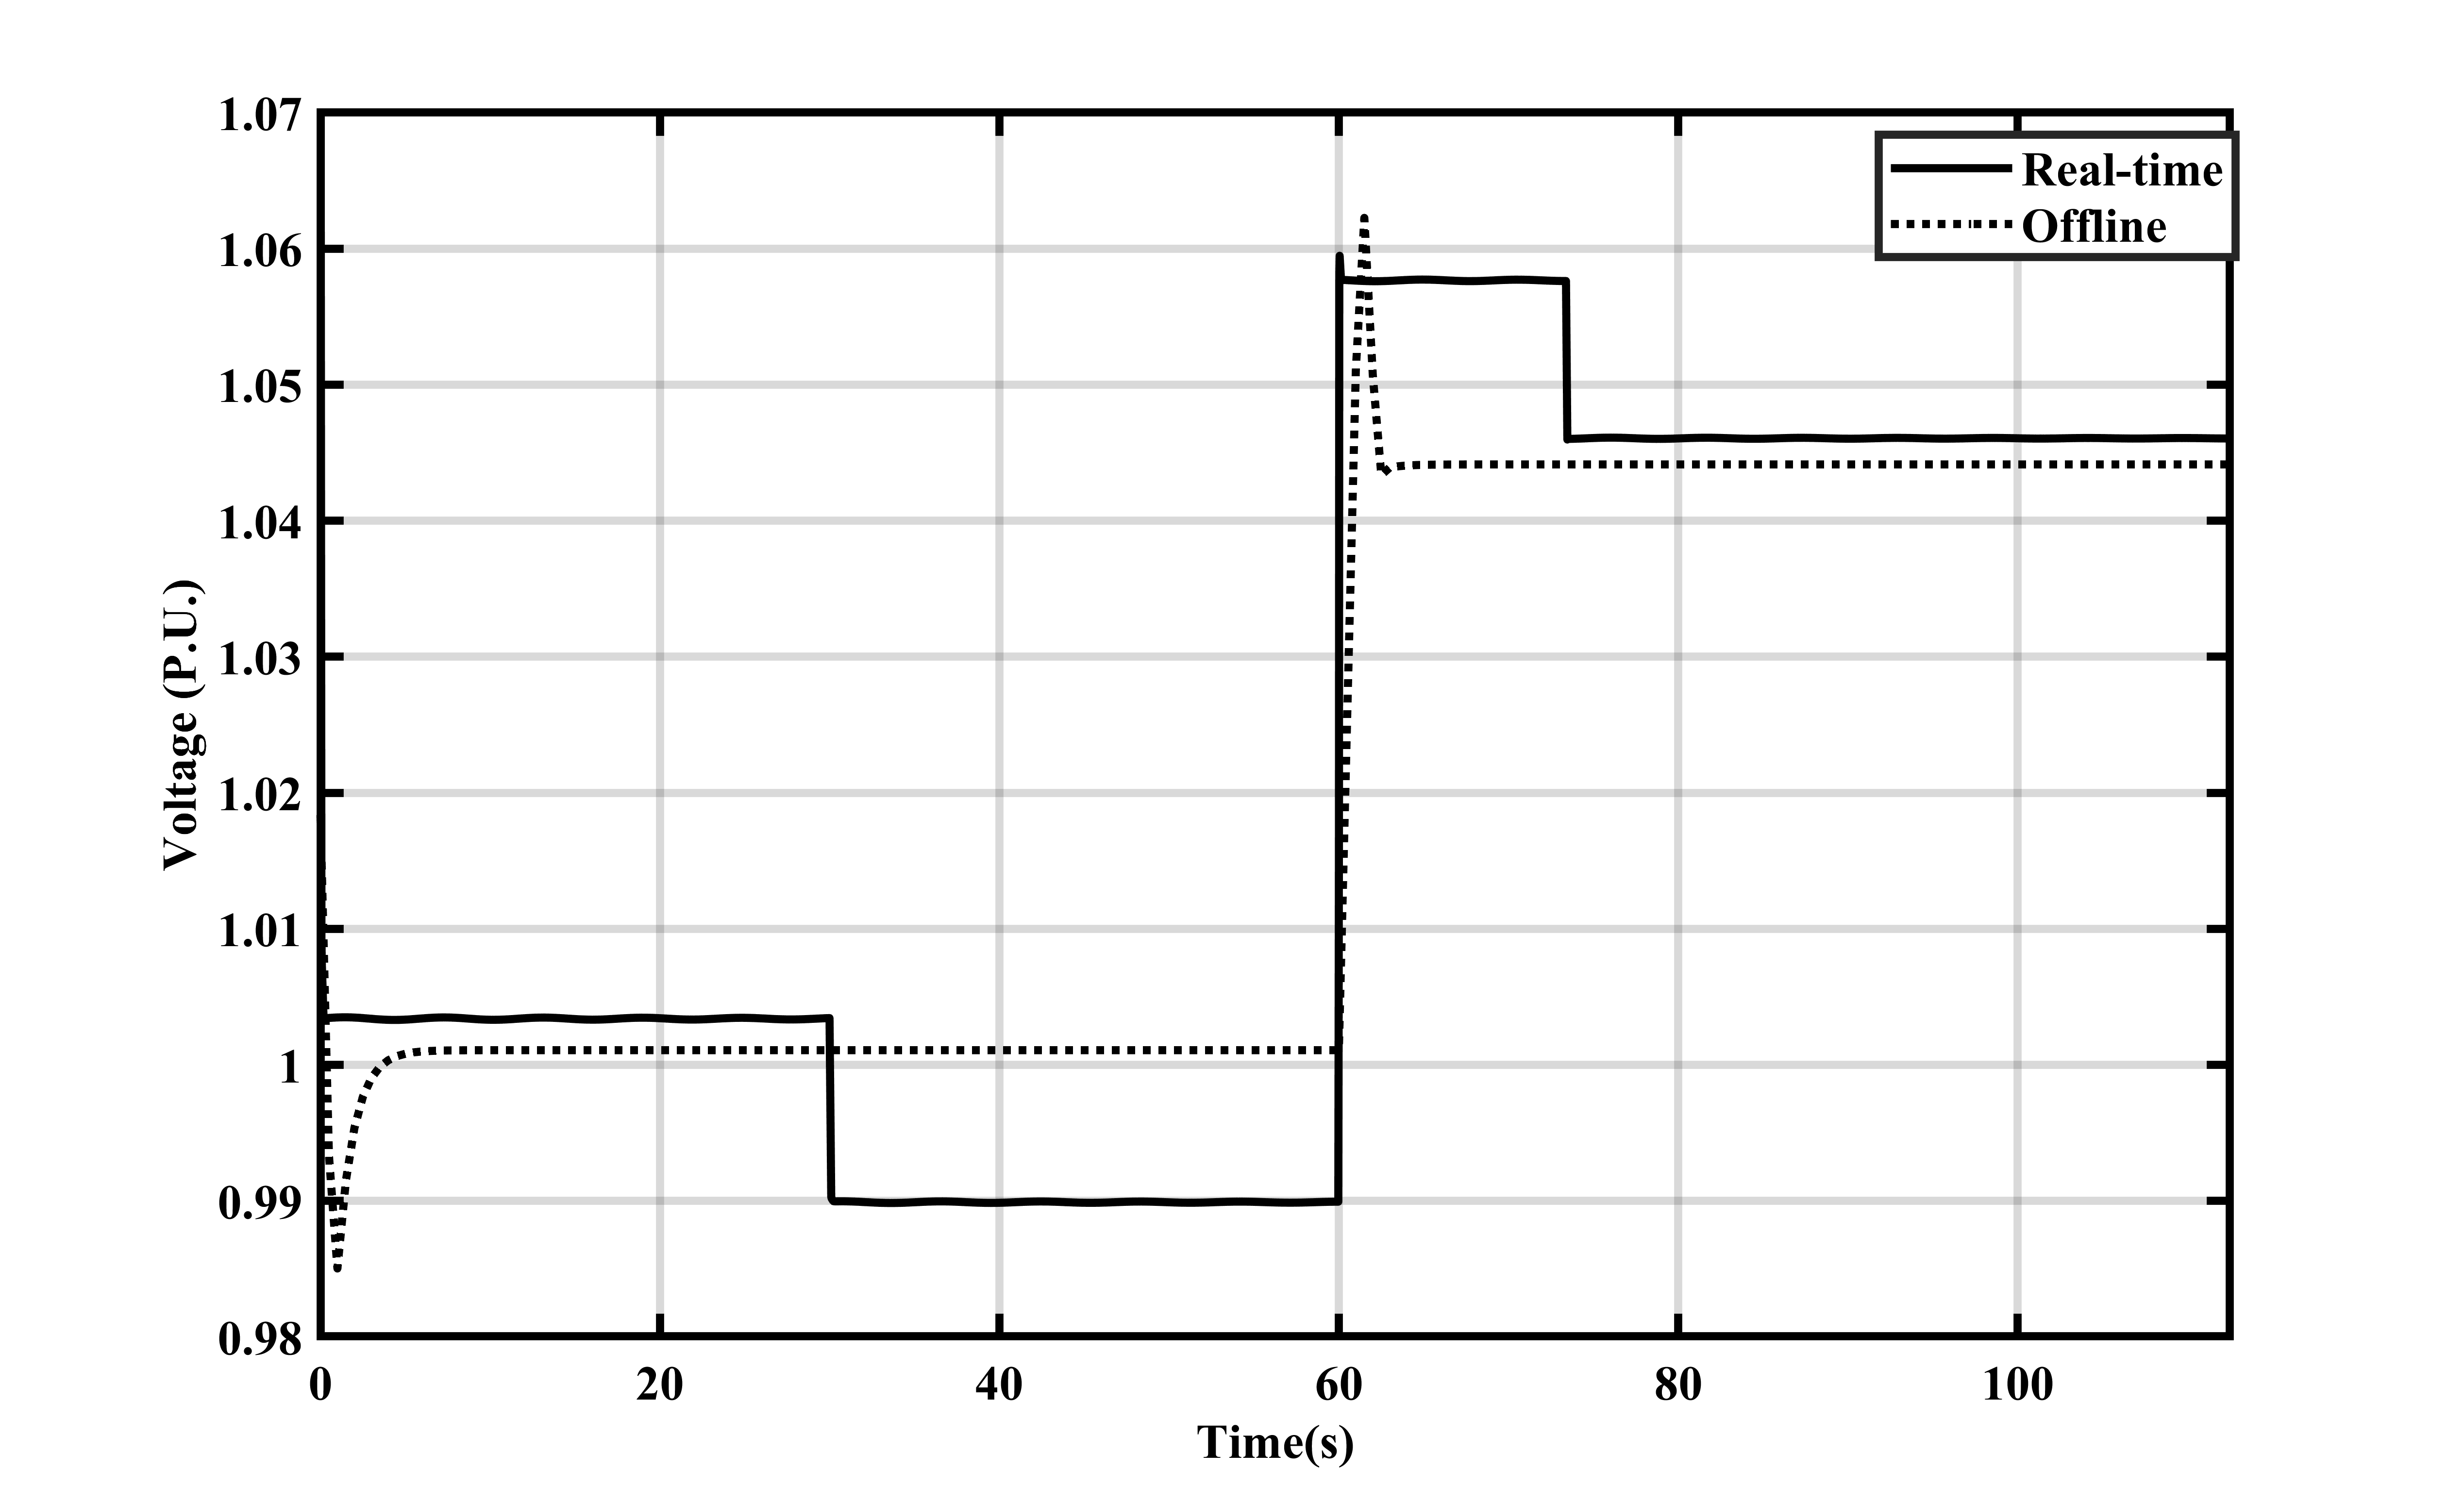
\includegraphics[width=\linewidth]{figs/OFF_VS_RT.png}
\caption{Real-time vs offline voltage profile with coordinated voltage control.}
\label{fig:RT_VS_OFF_V}
\end{figure}
Fig. \ref{RT_PQ} shows the reactive power supplied the PV in B20090P. The offline results are shown using the solid line and real-time results are represented using the dotted lines. The responses differ less than 2\% and real-time response is seen to take longer in this case as well. The delay is consistent with the delay seen in Fig. \ref{fig:RT_VS_OFF_V}.

\begin{figure}[!h]
\centering
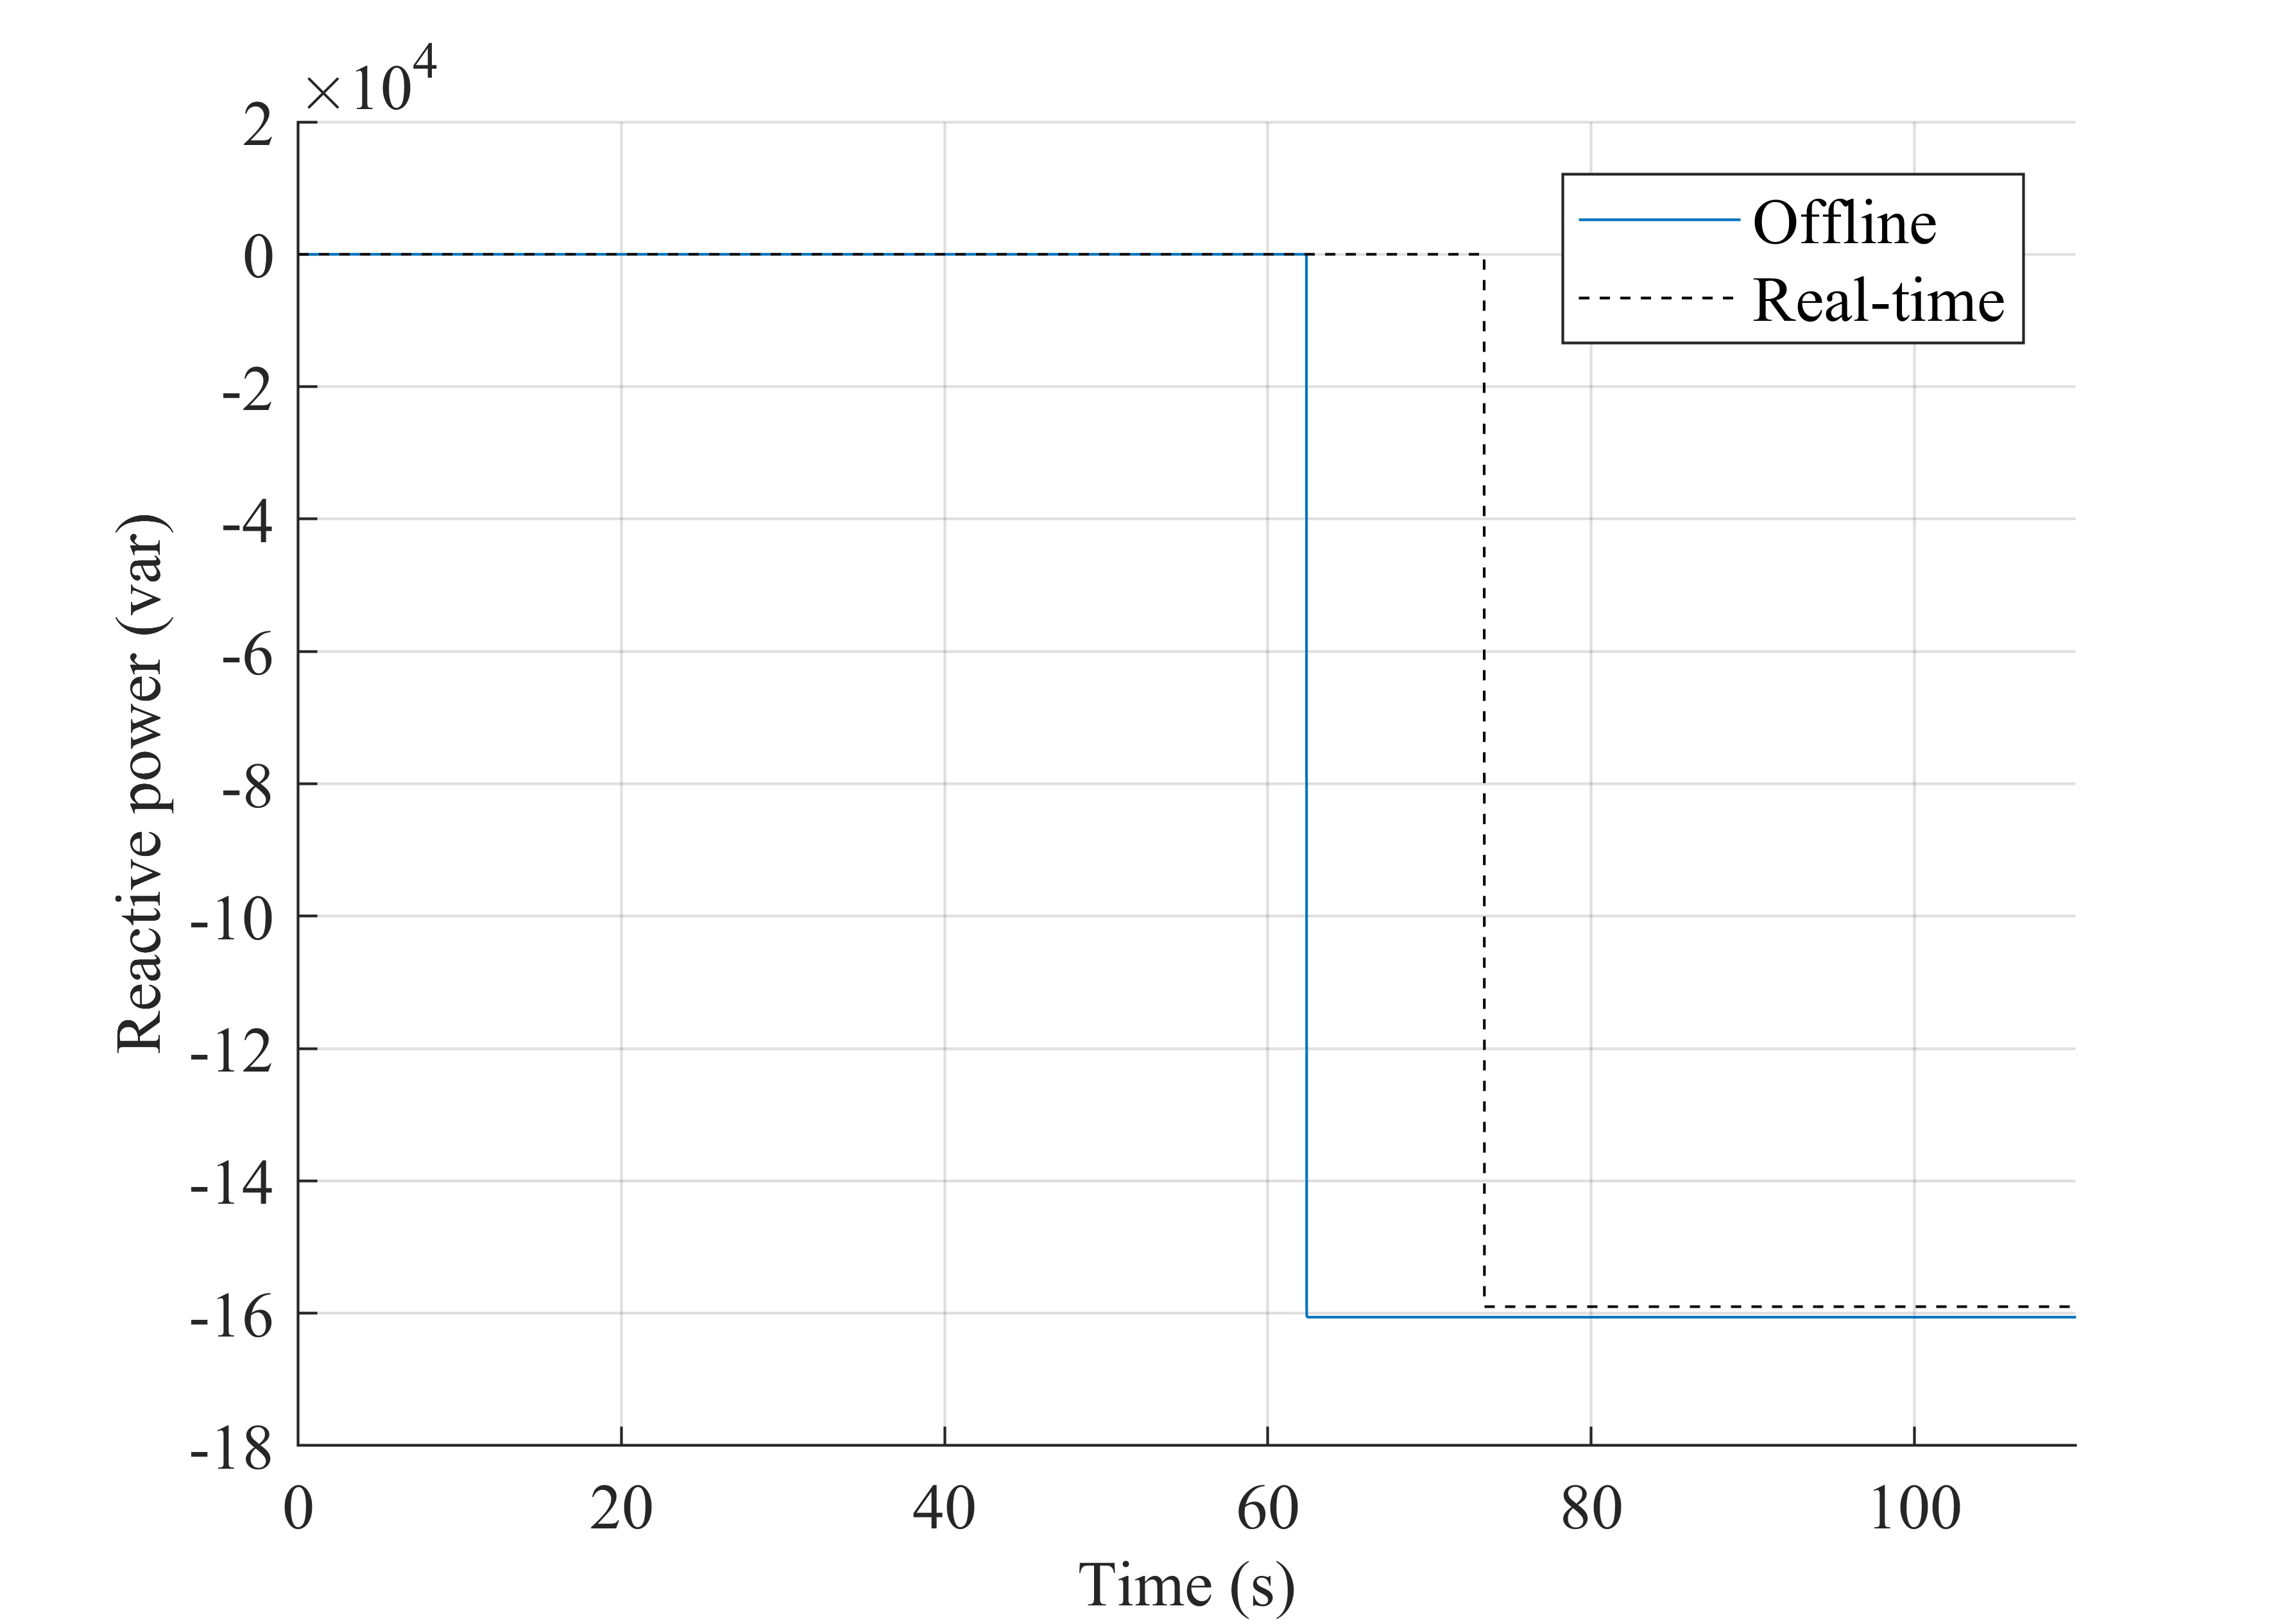
\includegraphics[width=\linewidth]{figs/PQ_RT.png}
\caption{Real-time vs off-line reactive power supplied by PV}
\label{fig:RT_PQ}
\end{figure}

Finally the switching operations of both CAP1 and CAP2 mentioned in Section \ref{off1} for both real-time and offline simulations are shown in Fig. \ref{fig:RT_CAP}. It can be seen that the resonances are the same but the real-time response takes 13s. This is also contestant with the results shown in Fig. \ref{fig:RT_VS_OFF_V}.

\begin{figure}[!h]
\centering
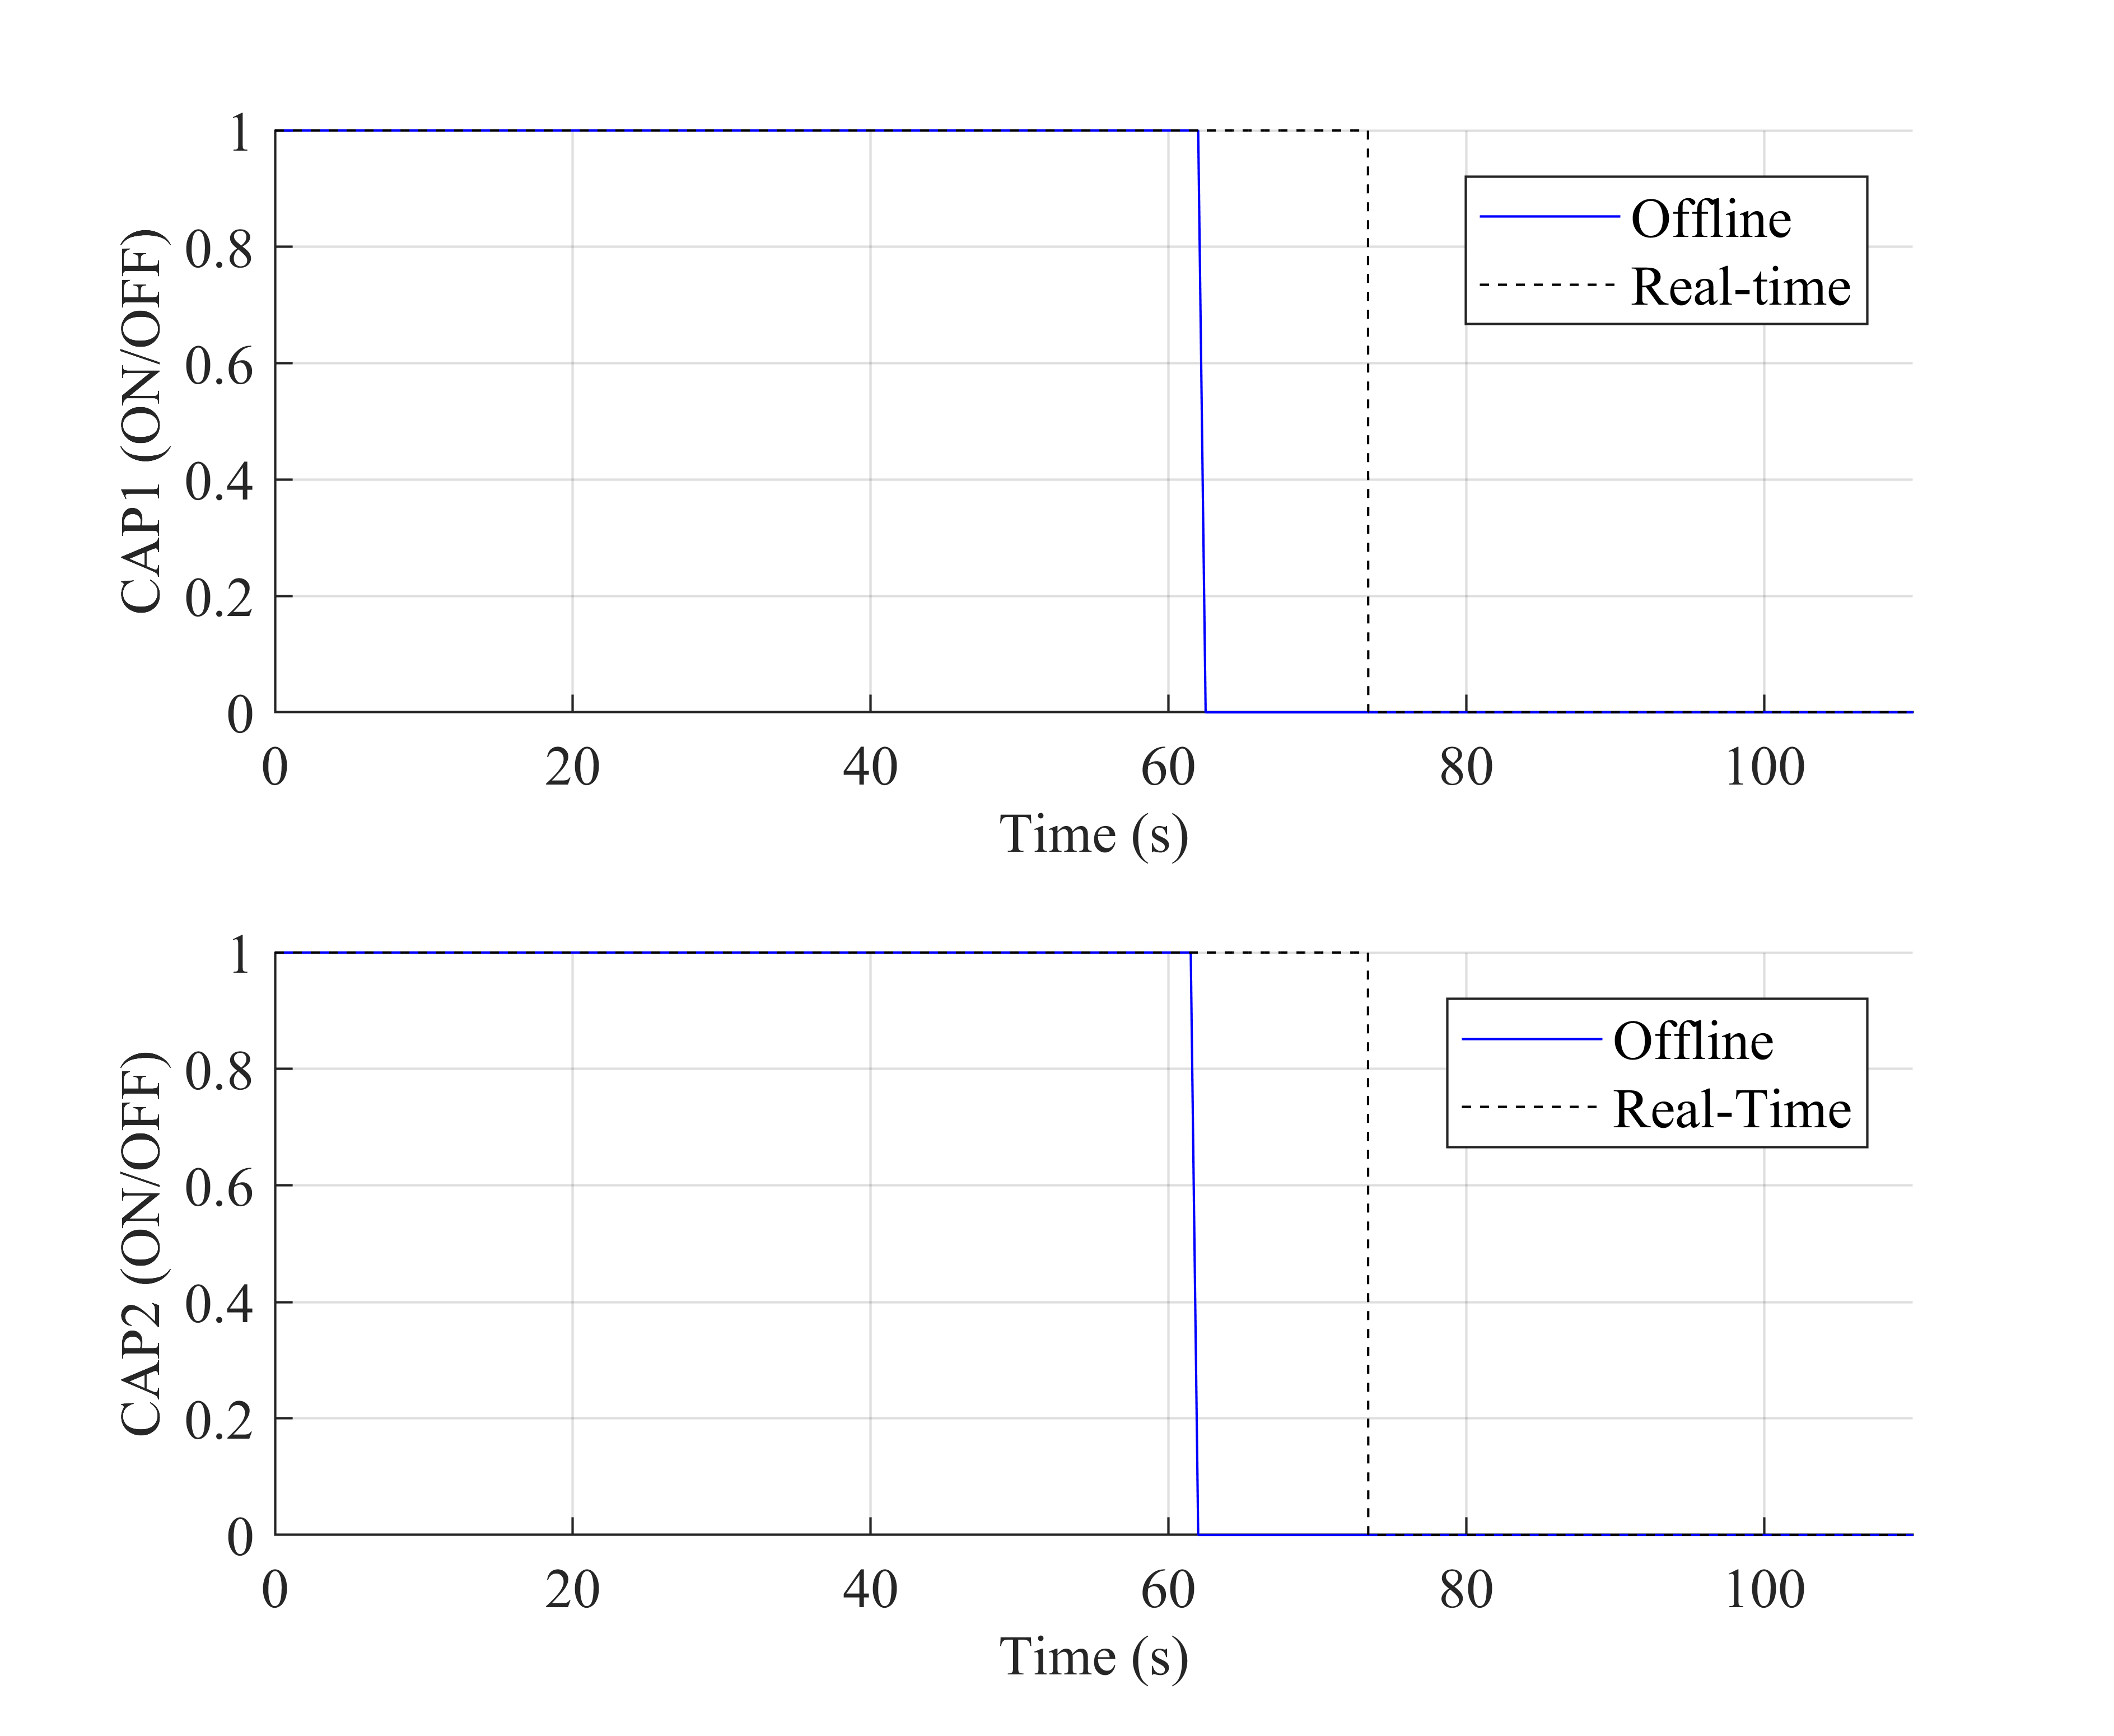
\includegraphics[width=\linewidth]{figs/CAPS_RT.PNG}
\caption{Capacitor bank switching states real-time vs offline.}
\label{fig:RT_CAP}
\end{figure}


\section{Conclusions}
In this paper, a coordinated voltage control algorithm was proposed to mitigate voltage violations on distribution systems with high penetration of distributed generations. The algorithm is capable of coordinating the inverter interfaced DGs with traditional regulation devices to keep the system voltage within acceptable limits. The algorithm was first validated using offline scenarios under ideal conditions. Then it was validated using real-time CHIL simulation, which was a more practical scenario comprised of estimated states and realistic communication structures. In both cases, the algorithm was shown to maintain the system voltage within acceptable ranges. 

\bibliographystyle{IEEEtran}
\bibliography{mybib.bib}


\end{document}


